%% abtex2-modelo-trabalho-academico.tex, v-1.8 laurocesar
%% Copyright 2012-2013 by abnTeX2 group at http://abntex2.googlecode.com/
%%
%% This work may be distributed and/or modified under the
%% conditions of the LaTeX Project Public License, either version 1.3
%% of this license or (at your option) any later version.
%% The latest version of this license is in
%%   http://www.latex-project.org/lppl.txt
%% and version 1.3 or later is part of all distributions of LaTeX
%% version 2005/12/01 or later.
%%
%% This work has the LPPL maintenance status `maintained'.
%%
%% The Current Maintainer of this work is the abnTeX2 team, led
%% by Lauro César Araujo. Further information are available on
%% http://abntex2.googlecode.com/
%%
%% This work consists of the files abntex2-modelo-trabalho-academico.tex,
%% abntex2-modelo-include-comandos and abntex2-modelo-references.bib
%%
 
% ------------------------------------------------------------------------
% ------------------------------------------------------------------------
% abnTeX2: Modelo de Trabalho Academico (tese de doutorado, dissertacao de
% mestrado e trabalhos monograficos em geral) em conformidade com
% ABNT NBR 14724:2011: Informacao e documentacao - Trabalhos academicos -
% Apresentacao
% ------------------------------------------------------------------------
% ------------------------------------------------------------------------

\documentclass[
  % -- opções da classe memoir --
  12pt,                                         % tamanho da fonte
  %openright,                                   % capítulos começam em pág ímpar (insere página vazia caso preciso)
  openany,
  %twoside,                                     % para impressão em verso e anverso. Oposto a oneside
  oneside,
  a4paper,                                      % tamanho do papel.
  % -- opções da classe abntex2 --
  %chapter=TITLE,                               % títulos de capítulos convertidos em letras maiúsculas
  %section=TITLE,                               % títulos de seções convertidos em letras maiúsculas
  %subsection=TITLE,                            % títulos de subseções convertidos em letras maiúsculas
  %subsubsection=TITLE,                         % títulos de subsubseções convertidos em letras maiúsculas
  % -- opções do pacote babel --
  english,                                      % idioma adicional para hifenização
  brazil,                                       % o último idioma é o principal do documento
  ]{abntex2}

% ---
% PACOTES
% ---
% ---
% Pacotes fundamentais
% ---
\usepackage{cmap}                               % Mapear caracteres especiais no PDF
\usepackage{lmodern}                            % Usa a fonte Latin Modern
\usepackage[T1]{fontenc}                        % Selecao de codigos de fonte.
\usepackage[utf8]{inputenc}                     % Codificacao do documento (conversão automática dos acentos)
\usepackage{lastpage}                           % Usado pela Ficha catalográfica
\usepackage{indentfirst}                        % Indenta o primeiro parágrafo de cada seção.
\usepackage[usenames,dvipsnames]{color}         % Controle das cores
\usepackage[usenames,dvipsnames,table]{xcolor}  % Para colorir textos
\usepackage{graphicx}                           % Inclusão de gráficos
\usepackage[activate={true,nocompatibility},final,babel=true,tracking=true,kerning=true,spacing=true,factor=1100,stretch=10,shrink=10]{microtype}
% ---
% Pacotes adicionais
% ---
%\usepackage{lipsum}                            % para geração de dummy text
%\usepackage[brazil, english]{babel}            % Gera tudo em Portugues-BR
%\usepackage{verbatim}                          % Suporte a comentarios extensos
%\usepackage{acronym}                           % Suporte a acronimos
%\usepackage{paralist}                          % provê o inparaenum environment -> Causa erros no ITEMIZE
%\usepackage[shortlabels]{enumitem}
%\usepackage{lipsum}
\usepackage{amsthm,amsfonts,amsmath}            % Simbolos matematicos
\usepackage{array}                              % usado para centralizar células de tabelas
\usepackage{capa-epusp-abntex2}                 % Customizacao da capa e folha de rosto para poli-usp
\usepackage{enumerate}                          % Enumerate em alg. romandos
\usepackage{enumitem}
\usepackage{epsf}                               % Read EPS figures
\usepackage{epstopdf}
\usepackage{float}                              % Usado para posicionar imagens
\usepackage[noredefwarn,acronym,toc,subentrycounter,seeautonumberlist]{glossaries}
\usepackage{lettrine}
\usepackage{listings}                           % Inclusao de listagens de computador
\usepackage{longtable}
\usepackage{multirow}                           % Tabelas com span de multiplas linhas
\usepackage{pdflscape}                          % usado para landscape de página
\usepackage[final]{pdfpages}                    % Para fazer o include de arquivos PDF
\usepackage{pgfgantt}                           % para geração de gráfico de gantt
\usepackage{rotating}
\usepackage{spverbatim}
\usepackage{tikz}                               % para desenhar
\PassOptionsToPackage{hyphens}{url}             %\usepackage[hyphens]{url} % pacote para adicionar URLs no texto
\usepackage{hyperref}
\usepackage{xifthen}                            % provê o ifthen com o isempty
\usepackage{xparse}                             % For dualentry glossary + acronym personalized command
%\usepackage{underscore}                         % Para adicionar underscores nas urls
% Dúvidas se precisa
\usepackage{adjustbox}
%\usepackage{booktabs}
\usepackage{varwidth}

% ---
% Pacotes de citações
% ---
\usepackage[brazilian,hyperpageref]{backref}   % Paginas com as citações na bibl
\usepackage[alf,abnt-url-package=url]{abntex2cite}  % Citações padrão ABNT

% ---
% CONFIGURAÇÕES DE PACOTES
% ---
% ---
% Configurações do pacote backref
% Usado sem a opção hyperpageref de backref
%\renewcommand{\backrefpagesname}{Citado na(s) página(s):~}
% Texto padrão antes do número das páginas
%\renewcommand{\backref}{}
% Define os textos da citação
%\renewcommand*{\backrefalt}[4]{
%  \ifcase #1 %
%    Nenhuma citação no texto.%
%  \or
%    Citado na página #2.%
%  \else
%    Citado #1 vezes nas páginas #2.%
%  \fi}%
% ---

% Configurações do pacote listings
\lstdefinestyle{customc}{
  belowcaptionskip=1\baselineskip,
  breaklines=true,
  frame=L,
  %xleftmargin=\parindent,
  xleftmargin=0pt,
  language=Python,
  showstringspaces=false,
  basicstyle=\footnotesize\ttfamily,
  keywordstyle=\bfseries\color{green!40!black},
  commentstyle=\itshape\color{purple!40!black},
  identifierstyle=\color{blue},
  stringstyle=\color{orange},
}
\lstset{extendedchars=\true}
\lstset{inputencoding=utf8}
\lstset{escapechar=@,style=customc}

%Corrigindo erro de URLs muito longas não quebrando linha
 \tolerance 1414
 \hbadness 1414
 \emergencystretch 1.5em
 \hfuzz 0.3pt
 \widowpenalty=10000
 \vfuzz \hfuzz
 \raggedbottom

% ---
% Comandos personalizados
% ---
%%%%%%%%%%%%%%%%%%%%%%%%%%%%%%%%%%%%%%%%%%%%
%%        Comandos Gerais do Projeto      %%
%%%%%%%%%%%%%%%%%%%%%%%%%%%%%%%%%%%%%%%%%%%%

%% Comando gerador de Siglas
%%%% #1 = Sigla
%%%% #2 = Por extenso
\newcommand{\sigla}[2]{\emph{#1}\ifthenelse{\isempty{#2}}{}{: #2}}

%% Comando de texto temporário
\newcommand{\temporario}[1]{\textcolor{red}{#1}}

%%Destaque no texto
\newcommand{\destaque}[1]{\emph{#1}}

%%Espaçamento vertical interno de células de tabela
\newcommand{\espacoVert}{\vspace{3pt}}

%%Cor Padrão de cabeçalhos de tabelas
\newcommand{\headerColor}{RoyalBlue!70!black!80}
\newcommand{\headerFontStyle}{\sffamily\bfseries\color{white}}
\newcommand{\headerCell}[1]{
  %\multicolumn{1}{c|}{\cellcolor{\headerColor}\textcolor{white}{\sffamily\bfseries{#1}}}
  \cellcolor{\headerColor}\textcolor{white}{\sffamily\bfseries{#1}}
}

\newcommand{\sptrans}{\textit{SPTrans}}
\hyphenation{SPTrans}
\newcommand{\gpssocial}{\textit{GPS Social}}
\newcommand{\bigdata}{\textit{Big Data}}
\newcommand{\trilhasp}{\textbf{\href{http://trilhasp.datapublika.com}{\#TrilhaSP}}}
\hyphenation{TrilhaSP}

%Needs xparse package
\DeclareDocumentCommand{\newdualentry}{ O{} O{} m m m m } {
  \newglossaryentry{gls-#3}{name={#5},text={#5\glsadd{#3}},
    description={#6},#1
  }
  \newacronym[see={[Glossary: ]{gls-#3}},#2]{#3}{#4}{#5\glsadd{gls-#3}}
}
%% Some shades
\definecolor{Dark}{gray}{0.2}
\definecolor{MedDark}{gray}{0.4}
\definecolor{Medium}{gray}{0.6}
\definecolor{Light}{gray}{0.8}

%Contador de numeração dos casos de uso
\newcounter{numcasodeuso}
%Sequencia de Eventos (Reiniciado a cada caso de uso)
\newcounter{indiceseqeventosCdU}
%Casos de Extensão (Reiniciado a cada caso de uso)
\newcounter{indiceextensaoCdU}
%Casos de Inclusão (Reiniciado a cada caso de uso)
\newcounter{indiceinclusaoCdU}

%Comando que cria um caso de uso e é usado internamente no ambiente
\newcommand{\criarcasodeuso}{%
    %\clearpage
    %\null \\
    %\hrule\ \\
    \hspace{-\parskip}\hspace{-\parindent}\textbf{Caso de uso UC\thenumcasodeuso :} \hypertarget{UC\thenumcasodeuso}{} \cmdNomeCasodeuso\\
    \null \\
    \textbf{Descrição:} \cmdDescCasodeuso\\
    \null \\
    \textbf{Evento iniciador:} \cmdEventoIniCasodeuso\\
    \null \\
    \textbf{Atores:} \cmdAtoresCasodeuso\\
    \null \\
    \textbf{Pré-condição:} \cmdPrecondCasodeuso\\
    \null \\
    \textbf{Sequência de eventos:} \cmdSeqEventosCasodeuso\\
    \null \\
    \textbf{Pós-condição:} \cmdPoscondCasodeuso\\
    \null \\
    \textbf{Extensão:} \cmdExtensaoCasodeuso\\
    \null \\
    \textbf{Inclusão:} \cmdInclusaoCasodeuso\\
    \null \\
    \textbf{Requisito:} \cmdRequisitoCasodeuso
    %\ \\ \hrule
    \clearpage
}

%Criação do ambiente Caso de Uso
\newenvironment{casodeuso}{%Zerando contadores
    \setcounter{indiceseqeventosCdU}{0}%
    \setcounter{indiceextensaoCdU}{0}%
    \setcounter{indiceinclusaoCdU}{0}%
    \stepcounter{numcasodeuso}%
}{\criarcasodeuso}

%Comandos internos
\newcommand{\cmdNomeCasodeuso}{}
%\newcommand{\cmdLabelCasodeuso}{}
\newcommand{\cmdDescCasodeuso}{}
\newcommand{\cmdEventoIniCasodeuso}{}
\newcommand{\cmdAtoresCasodeuso}{}
\newcommand{\cmdPrecondCasodeuso}{Nenhuma}
\newcommand{\cmdSeqEventosCasodeuso}{Nenhum}
\newcommand{\cmdPoscondCasodeuso}{Nenhuma}
\newcommand{\cmdExtensaoCasodeuso}{Nenhum}
\newcommand{\cmdInclusaoCasodeuso}{Nenhum}
\newcommand{\cmdRequisitoCasodeuso}{}
%%
%Comandos User Friendly de Casos de Uso
%
%Nome do Caso de Uso
\newcommand{\nomeCdU}[1]{\renewcommand{\cmdNomeCasodeuso}{#1}}
%Label
%\newcommand{\labelCdU}[1]{\renewcommand{\cmdLabelCasodeusp}{\label{#1}}}
%Descrição do Caso de Uso
\newcommand{\descricaoCdU}[1]{\renewcommand{\cmdDescCasodeuso}{#1}}
%Evento iniciador do caso de uso
\newcommand{\eventoiniciadorCdU}[1]{\renewcommand{\cmdEventoIniCasodeuso}{#1}}
%Atores do caso de uso
\newcommand{\atoresCdU}[1]{\renewcommand{\cmdAtoresCasodeuso}{#1}}
%Pré-condição do caso de uso
\newcommand{\precondicaoCdU}[1]{\renewcommand{\cmdPrecondCasodeuso}{#1}}
%Contagem de eventos
\newcommand{\contaeventoCdU}{%
    \stepcounter{indiceseqeventosCdU}
    \theindiceseqeventosCdU
}
%Sequencia de Eventos
\newcommand{\eventosCdU}[1]{
    \ifdefstring{\cmdSeqEventosCasodeuso}{Nenhum}{%
        \expandafter\renewcommand\expandafter\cmdSeqEventosCasodeuso\expandafter{%
            \\\null \hspace{.65cm}\contaeventoCdU. #1%
        }
    }{%
        \expandafter\renewcommand\expandafter\cmdSeqEventosCasodeuso\expandafter{%
            \cmdSeqEventosCasodeuso\\\null \hspace{.65cm}\contaeventoCdU. #1%
        }
    }
}
%Pós-condições
\newcommand{\poscondicaoCdU}[1]{\renewcommand{\cmdPoscondCasodeuso}{#1}}
%Contador de extensões do caso de uso
\newcommand{\contaextensaoCdU}{%
    \stepcounter{indiceextensaoCdU}
    \theindiceextensaoCdU
}
%Casos de uso de extensão
\newcommand{\extensaoCdU}[1]{
    \ifdefstring{\cmdExtensaoCasodeuso}{Nenhum}{%
        \expandafter\renewcommand\expandafter\cmdExtensaoCasodeuso\expandafter{\\\null \hspace{.65cm}\contaextensaoCdU. #1}
    }{%
        \expandafter\renewcommand\expandafter\cmdExtensaoCasodeuso\expandafter{%
            \cmdExtensaoCasodeuso\\\null \hspace{.65cm}\contaextensaoCdU. #1%
        }
    }
}
%Contador de casos de inclusão
\newcommand{\containclusaoCdU}{%
    \stepcounter{indiceinclusaoCdU}
    \theindiceinclusaoCdU
}
%Casos de uso de inclusão
\newcommand{\inclusaoCdU}[1]{
    \ifdefstring{\cmdInclusaoCasodeuso}{Nenhum}{%
        \expandafter\renewcommand\expandafter\cmdInclusaoCasodeuso\expandafter{\\\null \hspace{.65cm}\containclusaoCdU. #1}
    }{%
        \expandafter\renewcommand\expandafter\cmdInclusaoCasodeuso\expandafter{%
            \cmdInclusaoCasodeuso\\\null \hspace{.65cm}\containclusaoCdU. #1%
        }
    }
}
%Requisitos do caso de uso
\newcommand{\requisitoCdU}[1]{\renewcommand{\cmdRequisitoCasodeuso}{\hyperlink{#1}{#1}}}

%%%%%%%%%%%%%%%%%%%%%%%%%%%%%%%%%%%%%%%%%%%%%%%%%%%%%%%%%%%%%%%%%%%%%%%%%%%%%%%
%%                                DIAGRAMAS                                  %%
%%%%%%%%%%%%%%%%%%%%%%%%%%%%%%%%%%%%%%%%%%%%%%%%%%%%%%%%%%%%%%%%%%%%%%%%%%%%%%%
% PARÂMETROS:
%#1 = nome_da_imagem
%#2 = valor para escalar a imagem ('1' = 100% ; '0.5' = 50% ; etc)
%#3 = caption a ser utilizado na imagem/diagrama
%#4 = label a ser utilizada com a imagem/diagrama -> Não pode conter espaços!
%%%%%%
% USO
%Diagramas e imagens com página em formato retrato
%\diagramaRetrato{nome_imagem}{valor_escala}{texto_caption}{texto_label}{fonte}{nota}
\newcommand{\diagramaRetrato}[6]{
    \begin{figure}[htb]%
        \caption{#3\label{fig:#4}}%
        \begin{center}
            \includegraphics[scale=#2]{./imagens/#1}%
        \end{center}%
        \fonte{#5}%
        \ifthenelse{\isempty{#6}}{}{\nota{#6}}%
    \end{figure}%
}

%Diagramas e imagens com página em formato paisagem
%\diagramaRetrato{nome_imagem}{valor_escala}{texto_caption}{texto_label}{autoria}
\newcommand{\diagramaPaisagem}[6]{
    \begin{landscape}
	    \begin{figure}[H]%
	        \caption{#3\label{fig:#4}}%
	        \begin{center}
	            \includegraphics[scale=#2]{./imagens/#1}%
	        \end{center}%
	        \fonte{#5}%
	        \ifthenelse{\isempty{#6}}{}{\nota{#6}}%
	    \end{figure}%
    \end{landscape}
}
%%%%%%%%%%%%%%%%%%%%%%%%%%%%%%%%%%%%%%%%%%%%%%%%%%%%%%%%%%%%%%%%%%%%%%%%%%%%%%%
%%                                REQUISITOS                                 %%
%%%%%%%%%%%%%%%%%%%%%%%%%%%%%%%%%%%%%%%%%%%%%%%%%%%%%%%%%%%%%%%%%%%%%%%%%%%%%%%
%%%%%%%%%%%%%%%%%%%%%%%%%%%%%%%%%%%%%%%
%%              USO                  %%
%%%%%%%%%%%%%%%%%%%%%%%%%%%%%%%%%%%%%%%
%
%\begin{Requisito}
%    \ReqTipo{<ARGUMENTO 1>}
%    \ReqNome{<ARGUMENTO 2>}
%    \ReqLabel{<LABEL>}
%    \ReqDescr{<ARGUMENTO 3>}
%    \ReqPrioridade{<ARGUMENTO 4>}
%    \ReqStatus{<ARGUMENTO 5>}
%    \ReqEstabilidade{<ARGUMENTO 6>}
%    \ReqOrigem{<ARGUMENTO 7>}
%    \ReqRationale{<ARGUMENTO 8>}
%    \ReqAssoc{<ARGUMENTO 9>}
%\end{Requisito}
%
%%%%%%%%%%%%%%%%%%%%%%%%%%%%%%%%%%%%%%%
%%     DESCRIÇÃO DOS ARGUMENTOS      %%
%%%%%%%%%%%%%%%%%%%%%%%%%%%%%%%%%%%%%%%
%% *** Nenhum argumento pode conter caracteres especiais, como o 'underscore' ***
% <LABEL>: Label a ser usada para referencias internas do documento
% <ARGUMENTO 1>: TIPO: ´Funcional´ (funcional) ou ´Nao Funcional´ (nao funcional)
% <ARGUMENTO 2>: Nome do requisito
% <ARGUMENTO 3>: Descrição do Requisito
% <ARGUMENTO 4>: Prioridade [alta, media, baixa]
% <ARGUMENTO 5>: Status [proposto, aprovado, incorporado, validado]
% <ARGUMENTO 6>: Estabilidade [alta, media, baixa]
% <ARGUMENTO 7>: Origem [usuario, interna, externa]
% <ARGUMENTO 8>: Rationale - texto extenso
% <ARGUMENTO 9>: Requisitos Associados - por enquanto tem que listar na mão
%%%%%%%%%%%%%%%%%%%%%%%%%%%%%%%%%%%%%%%%%%%%%%%%%%%%%%%%%%%%%%%%%%%%%%%%%%%%%%%
%
%
% CONTADORES DOS REQUISITOS
\newcounter{indiceFuncional}
\newcounter{indiceNaoFuncional}
%
%
%% New job (that is, file)
\newwrite\ans
\immediate\openout\ans=tabRequisitos.aux
%
%
%% Usamos unexpanded... mas eu não sei porque. No meu
%% computador não funciona se removo o unexpanded. Acho
%% que deve ter algo haver com o `\\` dentro da expressão.
%% (Aliás, isso é muito provável, já que o significado
%% de `\\` é diferente no texto e em um ambiente tabular;
%% sua expansão tem que ser postergada para o momento em
%% que a tabela está sendo impressa (`PrintVolunteers`).
\newcommand{\AppendRequisito}[2]{%
    \immediate\write\ans{#1 & \expandafter#2 \unexpanded{\\}}%
}
%
\newcommand{\PrintRequisitos}{%
	\begin{tabular}{cl}%
	\hline
	\textbf{Identificação} & \textbf{Requisito} \\%
	\hline%
	\immediate\closeout\ans\input{tabRequisitos2.aux}%
	\hline%
	\end{tabular}%
}
%
%
%%%%%
\newenvironment{Requisito}{}{%
    \CriaRequisito%
}
%
%
% FUNÇÕES INTERNAS
\newcommand{\CmdReqTipo}{}%
\newcommand{\CmdReqLabel}{}%
\newcommand{\CmdReqNome}{}%
\newcommand{\CmdReqDescr}{}%
\newcommand{\CmdReqPrioridade}{}%
\newcommand{\CmdReqStatus}{}%
\newcommand{\CmdReqEstabilidade}{}%
\newcommand{\CmdReqOrigem}{}%
\newcommand{\CmdReqRationale}{}%
\newcommand{\CmdReqAssoc}{}%
%
%
%
%FUNÇÕES USER FRIENDLY
\newcommand{\ReqTipo}[1]{%
    \ifstrequal{#1}{funcional}{%
        \stepcounter{indiceFuncional}%
        \ReqLabel{RF\theindiceFuncional}%
        \renewcommand{\CmdReqTipo}{\multicolumn{3}{|l|}{\textbf{No:} RF\theindiceFuncional \hypertarget{\CmdReqLabel}{}} & (X) Funcional & ( ) Não Funcional \\}
    }{%
        \stepcounter{indiceNaoFuncional}%
        \ReqLabel{RNF\theindiceFuncional}%
        \renewcommand{\CmdReqTipo}{\multicolumn{3}{|l|}{\textbf{No:} RN\theindiceNaoFuncional} & ( ) Funcional & (X) Não Funcional \\}
    }
}
\newcommand{\ReqLabel}[1]{\renewcommand{\CmdReqLabel}{#1}}%
\newcommand{\ReqNome}[1]{\renewcommand{\CmdReqNome}{#1}}%
\newcommand{\ReqDescr}[1]{\renewcommand{\CmdReqDescr}{#1}}%
\newcommand{\ReqPrioridade}[1]{%
    \ifstrequal{#1}{alta}{%
        \renewcommand{\CmdReqPrioridade}{(X) Alta & ( ) Média & ( ) Baixa & \\}
    }{%
        \ifstrequal{#1}{media}{%
            \renewcommand{\CmdReqPrioridade}{( ) Alta & (X) Média & ( ) Baixa & \\}
        }{%
            \renewcommand{\CmdReqPrioridade}{( ) Alta & ( ) Média & (X) Baixa & \\}
        }
    }
}
\newcommand{\ReqStatus}[1]{
    \ifstrequal{#1}{proposto}{%
        \renewcommand{\CmdReqStatus}{(X) Proposto & ( ) Aprovado & ( ) Incorporado & ( ) Válido \\}
    }{
        \ifstrequal{#1}{aprovado}{%
            \renewcommand{\CmdReqStatus}{( ) Proposto & (X) Aprovado & ( ) Incorporado & ( ) Válido \\}
        }{
            \ifstrequal{#1}{incorporado}{%
                \renewcommand{\CmdReqStatus}{( ) Proposto & ( ) Aprovado & (X) Incorporado & ( ) Válido \\}
            }{
                \renewcommand{\CmdReqStatus}{( ) Proposto & ( ) Aprovado & ( ) Incorporado & (X) Válido \\}
            }%
        }%
    }
}%
\newcommand{\ReqEstabilidade}[1]{
    \ifstrequal{#1}{alta}{%
        \renewcommand{\CmdReqEstabilidade}{(X) Alta & ( ) Média & ( ) Baixa & \\}
    }{%
        \ifstrequal{#1}{media}{%
            \renewcommand{\CmdReqEstabilidade}{( ) Alta & (X) Média & ( ) Baixa & \\}
        }{%
            \renewcommand{\CmdReqEstabilidade}{( ) Alta & ( ) Média & (X) Baixa & \\}
        }
    }
}
\newcommand{\ReqOrigem}[1]{
    \ifstrequal{#1}{usuario}{%
        \renewcommand{\CmdReqOrigem}{(X) Usuário & ( ) Interna & ( ) Externa & \\}%
    }{%
        \ifstrequal{#1}{interna}{%
            \renewcommand{\CmdReqOrigem}{( ) Usuário & (X) Interna & ( ) Externa & \\}%
        }{
            \renewcommand{\CmdReqOrigem}{( ) Usuário & ( ) Interna & (X) Externa & \\}%
        }%
    }%
}
\newcommand{\ReqRationale}[1]{\renewcommand{\CmdReqRationale}{#1}}%
\newcommand{\ReqAssoc}[1]{\renewcommand{\CmdReqAssoc}{#1}}%
%
%
%Função Requisito - utilizada indiretamente pelo ambiente Requisito
\newcommand{\CriaRequisito}{
    \begin{table}[!h]
        \begin{tabular}{|lllll|}%
            \hline%
                \CmdReqTipo%
            \hline%
                \multicolumn{5}{|l|}{%
                    \begin{minipage}{1\textwidth}%
                        \espacoVert%
                        \textbf{Requisito:} \CmdReqNome%#2%
                        \espacoVert%
                    \end{minipage}%
                } \\%
            \hline%
                \multicolumn{5}{|l|}{%
                    \begin{minipage}{1\textwidth}%
                        \espacoVert%
                        \textbf{Descrição:} \CmdReqDescr%#3%
                        \espacoVert%
                    \end{minipage}%
                } \\%
            \hline%
                \textbf{Prioridade:} & \CmdReqPrioridade%
            \hline%
                \textbf{Status:} & \CmdReqStatus%
            \hline%
                \textbf{Estabilidade:} & \CmdReqEstabilidade%
            \hline%
                \textbf{Origem:} & \CmdReqOrigem%
            \hline%
                \multicolumn{5}{|l|}{%
                    \begin{minipage}{1\textwidth}%
                        \espacoVert%
                        \textbf{Rationale:} \CmdReqRationale%#8%
                        \espacoVert%
                    \end{minipage}%
                } \\%
            \hline%
                \multicolumn{5}{|l|}{%
                    \begin{minipage}{1\textwidth}%
                        \espacoVert%
                        \textbf{Requisitos Associados:} \CmdReqAssoc%#9%
                        \espacoVert%
                     \end{minipage}%
                 } \\%
             \hline%
        \end{tabular}
     \end{table}
    \AppendRequisito{\CmdReqLabel}{\CmdReqNome}
}% FIM DO COMMAND CriaRequisito
%


% ---
% Informações de dados para CAPA e FOLHA DE ROSTO
% ---
\titulo{\#TrilhaSP}
\autor{Diego Rabatone Oliveira}
\local{São Paulo}
\data{Dezembro/2014}
\orientador[Orientador:]{Prof. Dr. Reginaldo Arakaki}
\coorientador[Co-orientadora:]{Eng$^a$. Haydée Svab}
\instituicao{%
    Universidade de São Paulo -- USP
    \par
    Escola Politécnica - EP
    \par 
    Graduação em Engenharia Elétrica - Ênfase Computação}
\tipotrabalho{Monografia}
% O preambulo deve conter o tipo do trabalho, o objetivo,
% o nome da instituição e a área de concentração
\preambulo{Monografia apresentada à Escola Politécnica da Universidade de São Paulo para a Conclusão do Curso de Engenharia.}
\areaconcentracao{Engenharia Elétrica - Computação}

% ---

% ---
% Configurações de aparência do PDF final
% alterando o aspecto da cor azul
\definecolor{blue}{RGB}{41,5,195}

% informações do PDF
\makeatletter
\hypersetup{
  %pagebackref=true,
  pdftitle={\@title},
  pdfauthor={\@author},
  pdfsubject={\imprimirpreambulo},
  pdfcreator={LaTeX with abnTeX2},
  pdfkeywords={abnt}{latex}{abntex}{abntex2}{trabalho acadêmico},
  colorlinks=true,           % false: boxed links; true: colored links
  linkcolor=blue,            % color of internal links
  citecolor=blue,            % color of links to bibliography
  filecolor=magenta,         % color of file links
  urlcolor=blue,
  bookmarksdepth=4
}
\makeatother

% ---

% ---
% Espaçamentos entre linhas e parágrafos
% ---

% O tamanho do parágrafo é dado por:
\setlength{\parindent}{1.3cm}

% Controle do espaçamento entre um parágrafo e outro:
\setlength{\parskip}{0.2cm}  % tente também \onelineskip




% ---
% compila o indice
% ---
\makeindex
% ---
% Compila o Glossário de Acrônimos
\makeglossaries

\newacronym{rest}{REST}{\textit{Representational State Transfer}}
\newacronym{sgbd}{SGBD}{Sistema de Gerenciamento de Base de Dados}
\hyphenation{Django}%
\newglossaryentry{django}{%
    name=Django,%
    description={\'{e} um framework para desenvolvimento r\'{a}pido para web, escrito em Python, que utiliza o padr\~{a}o MVT}%
}%
\newglossaryentry{nginx}{%
    name=nginx,%
    description={\'{E} um dos servidore HTTP e de proxy reverso que mais tem ganho espa\c{c}o no mercado, em grande parte por seu elevado desempenho. Ele serve ainda como servidor de cache e permite trabalhar com \textit{load balance} entre diversos servidores}%
}%
\newglossaryentry{uwsgi}{%
    name=uWSGI,%
    description={\'{e} um servidor de aplica\c{c}\~{a}o para diversas linguagens de programa\c{c}\~{a}o, sendo Python uma delas, sendo que ele apresenta um dos melhores desempenhos}%
}%
\newglossaryentry{json}{%
    name=JSON,%
    description={acrônimo para ``\textit{JavaScript Object Notation}'', é um formato leve para intercâmbio de dados computacionais que foi proposto por Douglas Crockford e é descrito na \href{https://tools.ietf.org/html/rfc4627}{RFC 4627}}%
}%
\newdualentry{mvt}{MVT}{\textit{Model View Template}}{\textit{Design Pattern} utilizada no framework Django similar à tradicional MVC (Model View Controller)}
\newacronym{its}{ITS}{Intelligent Transport Systems}
\newdualentry{ipi}{IPI}{Imposto sobre Porudtos Industrializados}{imposto que incide sobre os produtos industrializados nacionais e estrangeiros no momento do desembaraço aduaneiro de produto de procedência estrangeira, ou a saída do produto do estabelecimento industrial ou equiparado a industrial}
\newdualentry{api}{API}{Application Programming Interface}{ou Interface de Programação de Aplicações ou Interface de Programação de Aplicativos, é um conjunto de rotinas e padrões estabelecidos por um software para a utilização das suas funcionalidades por aplicativos que não pretendem envolver-se em detalhes da implementação do software, mas apenas usar seus serviços}
\newdualentry{mvc}{MVC}{\textit{Model View Controller}}{\textit{Design Pattern} muito conhecida e introduzida por \textit{Erich Gamma} em 1995}
\newdualentry{drf}{DRF}{\textit{Django Rest Framework}}{Módulo do Django para criar e expor uma API REST}
\newdualentry{psa}{PSA}{\textit{Python Social Auth}}{Módulo do Django para permitir autenticação com redes sociais}


%\newdualentry{tdd}{TDD}{\textit{Test Driven Development}}{ ou, em português, Desenvolvimento Orientado a Testes é uma técnica de desenvolvimento de software que baseia em um ciclo curto de repetições no qual escreve-se primeiro um teste para uma determinada funcionalidade e em seguida o código que vai fazer o programa passar no teste}


\glsresetall
% ----
% Início do documento
% ----
\begin{document}

% Retira espaço extra obsoleto entre as frases.
\frenchspacing

% ----------------------------------------------------------
% ELEMENTOS PRÉ-TEXTUAIS
% ----------------------------------------------------------
\pretextual

% ---
% Capa
% ---
\imprimircapa
% ---

% ---
% Folha de rosto
% (o * indica que haverá a ficha bibliográfica)
% ---
\imprimirfolhaderosto
% ---

% ---
% Ficha Catalográfica
% OBS: Gerada pela biblioteca da EPUSP
% ---
%TODO
%\includepdf{Ficha_Catalografica}
% ---

% ---
% Agradecimentos
% ---
%\begin{agradecimentos}
%À minha família, que me deu todas as oportunidades para que eu chegasse a este momento e sempre esteve ao meu lado, me apoiando e confiando em mim. Obrigado Maria Júlia Rabatone Oliveira, Luiz Francisco Oliveira, Pedro Rabatone Oliveira e Paula Rabatone Oliveira.

À minha grande companheira Haydée Svab, que também me co-orientou neste trabalho, por todo seu amore e apoio incondicional, com elogios, abraços, broncas e orientações. Sou muito feliz por tê-la em minha vida, e que muitas outras experiências venham para somarmos e construirmos juntos.

À Daniela B. Silva e ao Pedro Markun, em nome da comunidade Transparência Hacker, que me abriu todo um mundo de colaboração e transformação de nossa sociedade, por meio do uso de tecnologia, mas sem tê-la como objetivo e única via.

Ao Leonardo Alexandre Ferreira Leite, Thiago Costa Paiva e Tássio Naia, em nome do PoliGNU, Grupo de Estudos de Software Livre da Poli-USP, que ajudei a fundar em 2009 e aonde pude aprender muito sobre compartilhamento, troca, colaboração, Software Livre, tecnologia, companheirismo e dedicação.

Às professores Cíntia Borges Margi, Maria Eugênia Boscov e ao professor Felipe Pait, por todo apoio dado ao PoliGNU e ao PoliGen, e por ajudarem a construir uma Escola melhor para todas e todos.

Ao Giuliano Salcas Olguin, Orientador Pedagógico da Escola Politénica, que de chefe se tornou um grande amigo, com quem tive muitas oportunidades de aprendizado e troca.

À Ângela Teresa Buscema, Assistente Técnico Acadêmico da Escola Politénica, uma verdadeira mãe de todos os politécnicos e politénicas.

Ao Guttember Nunes (Gutem), por todo apoio dado na reta final deste trabalho.

Ao Prof. Dr. João José Neto (JJ), por todas as horas de conversa, por todo conhecimento oferecido durante minha graduação, e por ser um grande exemplo.

E ao meu orientador, Prof. Dr. Reginaldo Arakaki, por todo aprendizado oferecido e pela confiança em meu trabalho e potencial.
%\end{agradecimentos}
% ---

% ---
% RESUMOS
% ---

% resumo em português
%\setlength{\absparsep}{18pt} % ajusta o espaçamento dos parágrafos do resumo
%\begin{resumo}
%\lettrine{A}{ presente monografia} descreve a implementação do aplicativo \trilhasp, um aplicativo que se propõe a melhorar o fluxo de informações entre usuário e prestador de serviço público de transporte, tanto fornecendo aos gestores avaliações do sistema realizadas pelos usuários quanto disponibilizando aos usuários informações para uma tomada de decisão mais consciente ao utilizar o sistema de transporte.
Com o \trilhasp~os usuários do sistema público de transporte poderão avaliar o serviço, segundo critérios qualitativos como ``o ônibus estava muito lotado'', ``fui bem atendido pelo motorista'' e ``o ônibus estava sujo''. A opção por estes critérios qualitativos se deu pois identificou-se que eles influenciam na decisão do usuário sobre o modo de transporte preferido e não são facilmente mensurados por meio de tecnologias de automação, como é o caso da velocidade e frequência dos ônibus. Essas avaliações, que podem ser positivas ou negativas numa escala contínua, permitirão a criação de indicadores por ônibus que poderão ser utilizados pelas autoridades para melhorar o serviço e também influenciar no sistema de remuneração das empresas prestadoras de serviço.
O módulo ``Mapa'' mostrará aos usuários um mapa com todos os usuários conectados, o que permitirá ao usuário optar por ir ou não para o ponto de ônibus num determinado horário usando a informação de demanda e ``lotação'' do ponto naquele momento, o que pode melhorar a distribuição da demanda no sistema, e levar a uma melhora do serviço prestado.
Por fim, o módulo ``game'' tem por objetivo tanto atrair e reter os usuários no aplicativo quanto ser uma solução educativa, levando ao usuário informações e vivência verossímeis à realidade do sistema de transporte, como custo de um ônibus, necessidade de manutenção, etc.
O projeto foi desenvolvido utilizando tecnologias livres e também terá seu código fonte distribuído livremente.

\vspace{\onelineskip}

\vfill

\noindent 

\textbf{Palavras-chaves}: Aplicativo móvel, transporte público, mobilidade, software livre, gps social, gamificação, geolocalização
%\end{resumo}

% resumo em inglês
%\begin{resumo}[Abstract]
%\lettrine{T}{his work} describes the implementation of the \trilhasp~application, that aims to improve the flow of information between users and service providers of the public transport system, so it can positively change the urban mobility of the city. It will allow the users to evaluate the service and also make available to the users crowdsourced information about other users so each user can take better decisions on how and when to use the system.%
%
\trilhasp~users will be able to evaluate the transport service based on qualitative criteria such as ``How crowded was the bus'' or ``Were you well attended by the bus driver and the collector?''. This qualitative criteria was chosen because it was identified that they influence the users choice of transport mode and they are not as easy to measure with technology and automation as speed of bus frequency. This evaluations can be positive or negative on a continuous scale and they will allow the creation of indexes per bus vehicle so they can be used to improve the service and also be part of service provides remuneration.%
%
The ``map'' module will show a map with all currently connected users. This will allow them to take a more precise decision on how to go to take the bus. If the bus stop are too crowded the user can just postpone and do other things before, like going to a gym or finish the current work. This could influence the demand in a way that makes the system more rational.%
%
There is also a ``game'' module, that aims both to engage the user on the app and also educate the user about the costs and needs of a transport system.%
%
This project was developed with free software and it's own source code are available as a Free Software (as in freedom).

\vspace{\onelineskip}

\vfill

\noindent 

\textbf{Keywords}: Public transport, mobile, mobility, free software, social gps, gamification, geolocalization
%\end{resumo}

% ---
% inserir lista de ilustrações
% ---
\pdfbookmark[0]{\listfigurename}{lof}
\listoffigures*
\cleardoublepage
% ---

% ---
% inserir lista de tabelas
% ---
\pdfbookmark[0]{\listtablename}{lot}
\listoftables*
\cleardoublepage
% ---

% ---
% inserir lista de abreviaturas e siglas
% ---
%%\begin{siglas}
%\newacronym{rest}{REST}{\textit{Representational State Transfer}}
\newacronym{sgbd}{SGBD}{Sistema de Gerenciamento de Base de Dados}
\hyphenation{Django}%
\newglossaryentry{django}{%
    name=Django,%
    description={\'{e} um framework para desenvolvimento r\'{a}pido para web, escrito em Python, que utiliza o padr\~{a}o MVT}%
}%
\newglossaryentry{nginx}{%
    name=nginx,%
    description={\'{E} um dos servidore HTTP e de proxy reverso que mais tem ganho espa\c{c}o no mercado, em grande parte por seu elevado desempenho. Ele serve ainda como servidor de cache e permite trabalhar com \textit{load balance} entre diversos servidores}%
}%
\newglossaryentry{uwsgi}{%
    name=uWSGI,%
    description={\'{e} um servidor de aplica\c{c}\~{a}o para diversas linguagens de programa\c{c}\~{a}o, sendo Python uma delas, sendo que ele apresenta um dos melhores desempenhos}%
}%
\newglossaryentry{json}{%
    name=JSON,%
    description={acrônimo para ``\textit{JavaScript Object Notation}'', é um formato leve para intercâmbio de dados computacionais que foi proposto por Douglas Crockford e é descrito na \href{https://tools.ietf.org/html/rfc4627}{RFC 4627}}%
}%
\newdualentry{mvt}{MVT}{\textit{Model View Template}}{\textit{Design Pattern} utilizada no framework Django similar à tradicional MVC (Model View Controller)}
\newacronym{its}{ITS}{Intelligent Transport Systems}
\newdualentry{ipi}{IPI}{Imposto sobre Porudtos Industrializados}{imposto que incide sobre os produtos industrializados nacionais e estrangeiros no momento do desembaraço aduaneiro de produto de procedência estrangeira, ou a saída do produto do estabelecimento industrial ou equiparado a industrial}
\newdualentry{api}{API}{Application Programming Interface}{ou Interface de Programação de Aplicações ou Interface de Programação de Aplicativos, é um conjunto de rotinas e padrões estabelecidos por um software para a utilização das suas funcionalidades por aplicativos que não pretendem envolver-se em detalhes da implementação do software, mas apenas usar seus serviços}
\newdualentry{mvc}{MVC}{\textit{Model View Controller}}{\textit{Design Pattern} muito conhecida e introduzida por \textit{Erich Gamma} em 1995}
\newdualentry{drf}{DRF}{\textit{Django Rest Framework}}{Módulo do Django para criar e expor uma API REST}
\newdualentry{psa}{PSA}{\textit{Python Social Auth}}{Módulo do Django para permitir autenticação com redes sociais}


%\newdualentry{tdd}{TDD}{\textit{Test Driven Development}}{ ou, em português, Desenvolvimento Orientado a Testes é uma técnica de desenvolvimento de software que baseia em um ciclo curto de repetições no qual escreve-se primeiro um teste para uma determinada funcionalidade e em seguida o código que vai fazer o programa passar no teste}


\glsresetall
%\end{siglas}
% ---

% ---
% inserir lista de símbolos
% ---
%\begin{simbolos}
%
%\end{simbolos}
% ---

% ---
% inserir o sumario
% ---
\pdfbookmark[0]{\contentsname}{toc}
\tableofcontents*
\cleardoublepage
% ---

% ----------------------------------------------------------
% ELEMENTOS TEXTUAIS
% ----------------------------------------------------------
\textual

%
% EXEMPLO COM IMAGEM
%
%
%\begin{figure}[H]
%  \centering
%    \caption{Ciclo Otto}
%    \setlength\fboxsep{1.1pt}
%    \setlength\fboxrule{0.3pt}
%    \fbox{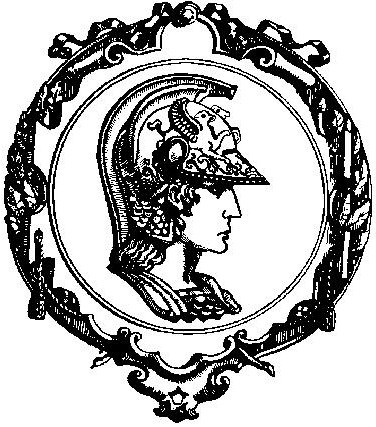
\includegraphics[width=10cm]{Figuras/otto.jpg}}
%    \legend{Fonte: \citeonline{ottofoto}}
%  \label{fig:otto}
%\end{figure}
%
%
%

% Capítulos
%Introdução - Bruno Fernandes
%$Rev$ - $Author$
%$Id$ - $Date$
% Rev5 - 09/12/13

\newpage
\chapter{Introdução}
\label{chp: Introdução}

\lettrine{A}{mobilidade urbana} é hoje um dos mais latentes problemas das grandes cidades de todo o mundo. Em 2010, considerando 439 áreas urbanas nos Estados Unidos, os congestionamentos fizeram com que os motoristas gastassem 4,8 bilhões de horas e comprassem 7.2 bilhões de litros de combustível além do necessário, a um custo de \$101 bilhões de dólares~\cite{Eisele2011}. Já em 2011, esses índices subiram para 5,5 bilhões de horas, 11 bilhões de litros de combustível e \$121 bilhões de dólares~\cite{Schrank2012}. Assim, percebe-se que não só identificam-se altos custos sociais, ambientais e econômicos, como também estes custos são crescentes.

A realidade brasileira não é muito diferente. De 2004 a 2007 o tempo de congestionamento de 4 das maiores cidades brasileiras (São Paulo, Rio de Janeiro, Belo Horizonte e Porto Alegre) cresceu a uma taxa anual média de 16\%~\cite{SOUSAPRRESENDE2009}. Se considerarmos ainda as políticas públicas de incentivo ao mercado automobilístico, mais especificamente a redução do \gls{ipi} para automóveis\footnote{\url{http://g1.globo.com/carros/noticia/2014/01/ipi-para-carros-sobe-partir-desta-quarta-e-deve-impactar-nos-precos.html} - último acesso em 19/06/2014} implementadas de maio de 2012 a dezembro de 2013, pode-se esperar que o crescimento do índice de congestionamento tenha sido até maior.

Para além dos congestionamentos, existem ainda outras externalidades comuns na área do transporte, como a poluição e os acidentes de trânsito\footnote{\url{http://repositorio.ipea.gov.br/bitstream/11058/2448/1/td_0586.pdf}}. Se elas têm suas medidas de desempenhos já consagradas e já se estuda sobre as deseconomias que as causam, a externalidade relativa à insatisfação do usuário do transporte público é terreno ainda pouco explorado na área de desenvolvimento de software. Sobram evidências de que há questionamentos quanto à qualidade do serviço prestado~\cite{Urbana-PE2010,Rodrigues,Rodrigues2006,Cellos2012}. “O reajuste das tarifas e a má qualidade do transporte público foram o estopim das manifestações de junho, que tomaram as ruas de várias capitais do país” afirma artigo publicado pelo IPEA\footnote{\url{http://www.ipea.gov.br/desafios/index.php?option=com_content&view=article&id=2972:catid=28&Itemid=23}} a respeito das manifestações que tomaram o país em 2013. Bastante polêmicas e controversas, mesmo assim ainda podendo ser entendidas sob esse prima, estão diversas queimas de ônibus como forma de protesto contra a má-qualidade do sistema. Estudo da ANTP\footnote{\url{http://www.antp.org.br/_5dotSystem/download/dcmDocument/2013/01/10/057A84C9-76D1-4BEC-9837-7E0B0AEAF5CE.pdf} } aponta como uma das recomendações para se combater as deseconomias do transporte público haver financiamentos de estudos e projetos para melhor caracterizar “condições atuais de transporte e trânsito para subsidiar projetos de melhoria”. Aqui este projeto encontra sua motivação e respaldo. Hoje, graças à emergência de recursos tecnológicos de comunicações que utilizam conceitos como redes, geolocalização, comunicação multidirecional e outros, pode-se definir processos que unam com facilidade os extremos das cadeias de transporte e, assim, permitir um melhor planejamento e correções de rumo mesmo durante a execução do planejamento do sistema de transporte, melhorando a sua eficiência tanto para o poder público, quanto para usuários e prestadores de serviço.
	
%\section{Contexto do Trabalho}\label{sec:contexto}
%\lipsum[3-4]
%\section{Motivação}\label{sec:motivação}

\section{Justificativa do projeto}\label{sec:justificativa}
	Atualmente já existem diversos aplicativos que trabalham, majoritariamente, trabalhando informações fornecidas pela SPTrans e oferecendo-as aos usuários. Isso se traduz em serviços de escolha de linha de ônibus, determinação de rotas e verificação de localização de ônibus com retorno também de quanto tempo é estimado para chegar num ponto específico. Não foi encontrado aplicativo que integrasse esse tipo de informação à coleta de avaliação dos usuários sobre elementos-chaves do sistema que não são automaticamente mensuráveis. Assim, além de oferecer a informação da SPTrans tratada, também será captada a opinião do usuário no momento do uso gerando informação de feed-back útil tanto para usuários e SPTrans como fiscalizadores, como para as operadoras terem melhor controle da qualidade de sua operação.

%\section{Objetivos}\label{sec:objetivos}

\subsection{Geral}\label{subsec:objGerais}
O objetivo geral do projeto é desenvolver um software que corrobore para a melhoria da mobilidade nas cidades pelo incremento da qualidade e da eficiência do sistema público de transporte urbano, mais especificamente rodoviário (ônibus). Será desenvolvido um produto considerando as condições de contorno da Região Metropolitana de São Paulo, que é o maior conglomerado urbano do Brasil com aproximadamente 20 milhões de habitantes. 

\subsection{Específicos}\label{subsec:objEspec}
São objetivos específicos do projeto: gerar dados e informações de valor para os atores envolvidos no sistema, a saber, operadores dos sistemas de transporte público, usuários e SPTrans; possibilitar a troca de informações triangular entre os três atores do sistema; corroborar para a eficiência do sistema pois com mais informação haverá mais controle de operação; promover transparência já que as informações geradas serão em sua maioria dados públicos sujeitos à Lei 12.527/2011; e estimular a conscientização para o usuário acerca do funcionamento do sistema público de transporte por ônibus.
	
\section{Escopo e critério de sucesso}\label{sec:Escopo}
	Ao final deste projeto o software contará com uma série de módulos, a saber:
	\begin{itemize}%[\itshape a\upshape)]
		\item módulo de avaliação do sistema de transporte;
		\item módulo de “gamificação” que terá as funções de oferecer um jogo que atraia e incentive a participação dos usuários e também sirva para um propósito pedagógico de conscientizar os usuários sobre a gestão de um sistema de transporte;
		\item módulo de “gps social”, que levantará informações de demanda do sistema de transporte e as fornecerá aos usuários em tempo real por meio de um mapa; e
		\item módulo de informações do sistema, que irá coletar as informações oferecidas pelo prestador de serviços (ex.: SPTrans) e disponibilizar à população – informações como tempo de espera de um ônibus, linhas que passam por um determinado ponto.
	\end{itemize}.

\section{Não-escopo}\label{sec:NãoEscopo}
	Não está no escopo de implementação deste projeto um ou mais módulos que permitam a integração do sistema com prestadores de serviço não ligados ao sistema de transporte, apesar de a arquitetura do sistema ser modelada para aceitar tais recursos num momento futuro.

%\section{Stakeholders}\label{sec:stakeholders}
%	Na matriz abaixo encontram-se os \emph{stakeholders} do projeto e seus respectivos poder e influência no projeto:
%
%	\bigskip
%	\begin{table}[H]
%	\centering
%	\caption{Stakeholders, relacionamento, interesse e poder}
%    \begin{tabular}{lccc}
%      \toprule
%      \headerCell{Parte interessada} &
%      \begin{minipage}{0.2\textwidth}
%        \espacoVert
%        \headerCell{Relacionamento com o Projeto}
%        \espacoVert
%      \end{minipage} &
%      \headerCell{Interesse (A/B)} &
%      \headerCell{Poder (A/B)}\\
%        
%      \midrule
%         
%			\textbf{Diego Rabatone Oliveira} &
%			Respons\'avel &
%			A &
%			A\\
%			
%			\textbf{Reginaldo Arakaki} &
%			Orientador &
%			A &
%			A\\
%
%			\textbf{Haydée Svab} &
%			Co-orientadora &
%			A &
%			A\\
%
%			\textbf{Prefeitura de São Paulo} &
%			Interessada &
%			B &
%			B\\
%			
%			\textbf{SPTrans} &
%			Interessada &
%			B &
%			B\\
%
%			\bottomrule
%	\end{tabular}
%	\end{table}

%\bigskip

\section{Restrições}\label{sec:restrições}
Todo desenvolvimento será realizado utilizando licenças livres e possiveis integrações com softwares terceiros devem levar este fato em consideração, ou seja, será preciso que haja compatibilidade de licenças.



\section{Objetivos}\label{sec:objetivos}

\subsection{Geral}\label{subsec:objGerais}
O objetivo geral do projeto é desenvolver um software que corrobore para a melhoria da mobilidade nas cidades pelo incremento da qualidade e da eficiência do sistema público de transporte urbano, mais especificamente rodoviário (ônibus). Será desenvolvido um produto considerando as condições de contorno da Região Metropolitana de São Paulo, que é o maior conglomerado urbano do Brasil com aproximadamente 20 milhões de habitantes. 

\subsection{Específicos}\label{subsec:objEspec}
São objetivos específicos do projeto: gerar dados e informações de valor para os atores envolvidos no sistema, a saber, operadores dos sistemas de transporte público, usuários e SPTrans; possibilitar a troca de informações triangular entre os três atores do sistema; corroborar para a eficiência do sistema pois com mais informação haverá mais controle de operação; promover transparência já que as informações geradas serão em sua maioria dados públicos sujeitos à Lei 12.527/2011; e estimular a conscientização para o usuário acerca do funcionamento do sistema público de transporte por ônibus.
	
\section{Escopo e critério de sucesso}\label{sec:Escopo}
	Ao final deste projeto o software contará com uma série de módulos, a saber:
	\begin{itemize}%[\itshape a\upshape)]
		\item módulo de avaliação do sistema de transporte;
		\item módulo de “gamificação” que terá as funções de oferecer um jogo que atraia e incentive a participação dos usuários e também sirva para um propósito pedagógico de conscientizar os usuários sobre a gestão de um sistema de transporte;
		\item módulo de “gps social”, que levantará informações de demanda do sistema de transporte e as fornecerá aos usuários em tempo real por meio de um mapa; e
		\item módulo de informações do sistema, que irá coletar as informações oferecidas pelo prestador de serviços (ex.: SPTrans) e disponibilizar à população – informações como tempo de espera de um ônibus, linhas que passam por um determinado ponto.
	\end{itemize}

\section{Não-escopo}\label{sec:NãoEscopo}
	Não está no escopo de implementação deste projeto um ou mais módulos que permitam a integração do sistema com prestadores de serviço não ligados ao sistema de transporte, apesar de a arquitetura do sistema ser modelada para aceitar tais recursos num momento futuro.

%\section{Stakeholders}\label{sec:stakeholders}
%	Na matriz abaixo encontram-se os \emph{stakeholders} do projeto e seus respectivos poder e influência no projeto:
%
%	\bigskip
%	\begin{table}[H]
%	\centering
%	\caption{Stakeholders, relacionamento, interesse e poder}
%    \begin{tabular}{lccc}
%      \toprule
%      \headerCell{Parte interessada} &
%      \begin{minipage}{0.2\textwidth}
%        \espacoVert
%        \headerCell{Relacionamento com o Projeto}
%        \espacoVert
%      \end{minipage} &
%      \headerCell{Interesse (A/B)} &
%      \headerCell{Poder (A/B)}\\
%        
%      \midrule
%         
%			\textbf{Diego Rabatone Oliveira} &
%			Respons\'avel &
%			A &
%			A\\
%			
%			\textbf{Reginaldo Arakaki} &
%			Orientador &
%			A &
%			A\\
%
%			\textbf{Haydée Svab} &
%			Co-orientadora &
%			A &
%			A\\
%
%			\textbf{Prefeitura de São Paulo} &
%			Interessada &
%			B &
%			B\\
%			
%			\textbf{SPTrans} &
%			Interessada &
%			B &
%			B\\
%
%			\bottomrule
%	\end{tabular}
%	\end{table}

%\bigskip

\section{Restrições}\label{sec:restrições}
Todo desenvolvimento será realizado utilizando licenças livres e possiveis integrações com softwares terceiros devem levar este fato em consideração, ou seja, será preciso que haja compatibilidade de licenças.

%
%
%\section{Organização do trabalho}\label{sec:organização}
%
%	O presente projeto foi organizado nas etapas destacadas abaixo, iniciando-se com o desenvolvimento do \textit{hardware} e seguindo com o desenvolvimento do \textit{firmware} e do \textit{software}:
%	
%	\begin{itemize}
%		\item Concepção e validação do novo \textit{hardware}, implementado com novos microcontroladores e novos recursos;
%		\item Desenvolvimento de \textit{firmware} para controle de posição da VB, com testes em bancada;
%		\item Desenvolvimento de \textit{firmware} para controle dos instantes de acionamento da injeção e ignição, com testes em bancada;
%		\item Desenvolvimento de \textit{firmware} para aquisição de dados dos sensores;
%		\item Desenvolvimento de \textit{software} de monitoramento, que recebe e exibe na tela todas as informações de sensores e variáveis de erro do sistema, bem como tempos de atuação e a rotação calculada;
%		\item Aperfeiçoamento de \textit{firmware} para leitura de sensores e cálculo da variável final associada ao valor de tensão lido, tomando como referência para este cálculo a curva característica do sensor;
%		\item Aperfeiçoamento de \textit{software} de monitoramento, com implementação do pedal simulado para controle do motor diretamente do computador;
%		\item Aperfeiçoamento de \textit{firmware} para cálculos mais precisos dos sinais de atuação (injeção e ignição);
%		\item Aperfeiçoamento de \textit{firmware} para cálculo do tempo de injeção com base na massa de ar estimada;
%		\item Desenvolvimento de \textit{firmware} para controle de relés;
%		\item Desenvolvimento de \textit{firmware} para controle de rotação, com testes em bancada;
%		\item Testes finais no veículo, aplicado em dinamômetro inercial a fim de avaliar o desempenho do motor em condições de carga.
%	\end{itemize}

\section{Planejamento}\label{sec:planejamento}
\subsection{Escopo, Cronograma e Orçamento da EAP}\label{subsec:eap}
%\diagramaRetrato{EAP_2.pdf}{1}{EAP, cronograma e orçamento}{eap2}
Os itens \textit{1.2.2} e \textit{1.3} da Estrutura Analítica de Projeto dizem respeito às atividades do segundo semestre e por este motivo não foram completamente definidas/planejadas.\\
A previsão de horas de trabalho (HT) está na coluna \textit{Trabalho} da tabela \ref{tab:eapwbs}.\\
\begin{table}[H]
  \centering
  \caption {EAP/WBS}
    \begin{tabular}{llllll}
      \toprule

       \headerCell{EAP} & \headerCell{Nome} & \headerCell{Trabalho}  \\

      \midrule
      
      1        & TCC - \#TrilhaSP                          & 24d       \\
      1.1      & Documentação e especificação              & 20d 2h    \\
      1.1.1    & Definir Objetivos do projeto              & 3h        \\
      1.1.2    & Elaborar documento inicial                & 4h        \\
      1.1.3    & Realizar orçamento (HT) da EAP            & 2h        \\
      1.1.4    & Definir riscos do projeto                 & 5h        \\
      1.1.5    & Análise SWOT                              & 6h        \\
      1.1.6    & Levantar projetos existentes              & 3d 2h     \\
      1.1.6.1  & Lista de projetos                         & 6h        \\
      1.1.6.2  & Características dos projetos              & 2d        \\
      1.1.6.3  & Consolidar quadro de características      & 4h        \\
      1.1.7    & Definição dos módulos do projeto          & 1d 4h     \\
      1.1.7.1  & Módulos para os usuários                  & 1d        \\
      1.1.7.2  & Módulos para o Poder Público              & 4h        \\
      1.1.8    & Especificação dos módulos do projeto      & 7d        \\
      1.1.8.1  & Requisitos Funcionais                     & 2d        \\
      1.1.8.2  & Requisitos Não-Funcionais                 & 2d        \\
      1.1.8.3  & Modelagem de dados dos módulos            & 3d        \\
      1.1.9    & Especificação da Arquitetura              & 6d        \\
      1.1.9.1  & Estimativa de demanda de recursos         & 2d        \\
      1.1.9.2  & Levantamento de opções de infraestrutura  & 1d        \\
      1.1.9.3  & Definição da infraestrutura               & 2d        \\
      1.1.9.4  & Especificação de Infraestrutura           & 1d        \\
      1.2      & Relatórios e Apresentações                & 3d 6h     \\
      1.2.1    & 1o Semestre                               & 3d 6h     \\
      1.2.1.1  & Relatório Inicial 1sem                    & 2h        \\
      1.2.1.2  & Relatório Intermediário 1 (Abril)         & 3h        \\
      1.2.1.3  & Relatório Intermediário 2 (Maio)          & 3h        \\
      1.2.1.4  & Apresentação Intermediária 1sem           & 3h        \\
      1.2.1.5  & Relatório Final (Junho)                   & 2d        \\
      1.2.1.6  & Apresentação Final 1sem                   & 3h        \\
      1.2.2    & 2o Semestre                               & ~         \\
%      1.2.2.1  & Relatório Inicial 2sem                    & ~         \\
%      1.2.2.2  & Relatório Intermediário 1 (Setembro)      & ~         \\
%      1.2.2.3  & Relatório Intermediário 2 (Outubro)       & ~         \\
%      1.2.2.4  & Apresentação Intermediária 2sem           & ~         \\
%      1.2.2.5  & Relatório Final (Novembro)                & ~         \\
%      1.2.2.6  & Apresentação Final 2sem                   & ~         \\
      1.3      & Codificação                               & ~         \\
      1.3.1    & Prototipação (Mocks)                      & ~         \\
      1.3.1.1  & Protótipos de cada módulo                 & ~         \\
      1.3.1.2  & Design da interface                       & ~         \\
      1.3.2    & Produto Final (MVP)                       & ~         \\
      
      \bottomrule
    \end{tabular}
  \label{tab:eapwbs}
\end{table}
%\diagramaPaisagem{EAP_1.pdf}{0.9}{EAP e Linha do Tempo}{eap1}

\begin{landscape}
  \begin{figure}[ftbp]
  \caption{Gráfico de Gantt da EAP}
  \begin{center}
  \begin{ganttchart}[
    hgrid,
    vgrid,
    x unit=2.55mm,
    y unit title=0.35cm,
    y unit chart=0.52cm,
    %compress calendar,
    time slot format=isodate,
    title/.append style={draw=none, fill=\headerColor},
    title label font=\headerFontStyle,
    title label node/.append style={below=-1.6ex},
    title left shift=.05,
    title right shift=-.05,
    title height=1,
    bar/.append style={draw=none, fill=OliveGreen!75},
    bar label font=\footnotesize\color{black!50},
    bar incomplete/.append style={fill=Maroon},
    bar height=.2,
    bar top shift=.1,
    bar progress label node/.append style={above=3pt, right=2mm},
    group right shift=0,
    group top shift=.4,
    group height=.2,
    group peaks height=.2,
    %progress=today,
    %today=2014-05-04,
    %bar/.append style={fill=green},
    %bar progress label node/.append style={above=3pt, right=2mm}
  ]{2014-04-01}{2014-06-20}
  \gantttitlecalendar{month=name, week} \\
      \ganttgroup{\footnotesize{1}}{2014-04-2}{2014-06-18}\\ %TCC - \#TrilhaSP
      \ganttgroup{\footnotesize{1.1}}{2014-04-2}{2014-05-27}\\ %Documentação e especificação
      \ganttlinkedbar[progress=100]{\footnotesize{1.1.1}}{2014-04-2}{2014-04-2}\\ %Definir Objetivos do projeto
      \ganttlinkedbar[progress=100]{\footnotesize{1.1.2}}{2014-04-2}{2014-04-2}\\ %Elaborar documento inicial
      \ganttlinkedbar[progress=100]{\footnotesize{1.1.3}}{2014-04-2}{2014-04-3}\\ %Realizar orçamento (HT) da EAP
      \ganttlinkedbar{\footnotesize{1.1.4}}{2014-04-28}{2014-04-28}\\ %Definir riscos do projeto
      \ganttlinkedbar{\footnotesize{1.1.5}}{2014-04-28}{2014-04-29}\\ %Análise SWOT
      %\ganttgroup{\footnotesize{1.1.6}}{2014-04-29}{2014-05-2}\\ %Levantar projetos existentes
      \ganttlinkedbar[progress=80]{\footnotesize{1.1.6.1}}{2014-04-29}{2014-04-30}\\ %Lista de projetos
      %\ganttlink[link type=fin-to-sta]{elem6}{elem8}
      \ganttlinkedbar{\footnotesize{1.1.6.2}}{2014-04-30}{2014-05-2}\\ %Características dos projetos
      \ganttlinkedbar{\footnotesize{1.1.6.3}}{2014-05-2}{2014-05-2}\\ %Consolidar quadro de características
      %\ganttgroup{\footnotesize{1.1.7}}{2014-05-2}{2014-05-6}\\ %Definição dos módulos do projeto
      \ganttlinkedbar[progress=10]{\footnotesize{1.1.7.1}}{2014-05-2}{2014-05-5}\\ %Módulos para os usuários
      \ganttlinkedbar[progress=25]{\footnotesize{1.1.7.2}}{2014-05-5}{2014-05-6}\\ %Módulos para o Poder Público
      %\ganttgroup{\footnotesize{1.1.8}}{2014-05-6}{2014-05-15}\\ %Especificação dos módulos do projeto
      \ganttlinkedbar{\footnotesize{1.1.8.1}}{2014-05-6}{2014-05-8}\\ %Requisitos Funcionais
      \ganttlinkedbar{\footnotesize{1.1.8.2}}{2014-05-8}{2014-05-12}\\ %Requisitos Não-Funcionais
      \ganttlinkedbar{\footnotesize{1.1.8.3}}{2014-05-12}{2014-05-15}\\ %Modelagem de dados dos módulos
      %\ganttgroup{\footnotesize{1.1.9}}{2014-05-19}{2014-05-27}\\ %Especificação da Arquitetura
      \ganttlinkedbar[name=1191]{\footnotesize{1.1.9.1}}{2014-05-19}{2014-05-21}\\ %Estimativa de demanda de recursos
      \ganttlinkedbar{\footnotesize{1.1.9.2}}{2014-05-21}{2014-05-22}\\ %Levantamento de opções de infraestrutura
      \ganttlinkedbar{\footnotesize{1.1.9.3}}{2014-05-22}{2014-05-26}\\ %Definição da infraestrutura
      \ganttlinkedbar[name=1194]{\footnotesize{1.1.9.4}}{2014-05-26}{2014-05-27}\\ %Especificação de Infraestrutura
      \ganttgroup{\footnotesize{1.2}}{2014-05-2}{2014-06-18}\\ %Relatórios e Apresentações
      %\ganttgroup{\footnotesize{1.2.1}}{2014-05-2}{2014-06-18}\\ %1o Semestre
      \ganttbar[progress=100,name=1211]{\footnotesize{1.2.1.1}}{2014-05-2}{2014-05-2}\\ %Relatório Inicial 1sem
      \ganttlinkedbar[progress=90]{\footnotesize{1.2.1.2}}{2014-05-28}{2014-05-28}\\ %Relatório Intermediário 1 (Abril)
      \ganttlinkedbar{\footnotesize{1.2.1.3}}{2014-05-19}{2014-05-19}\\ %Relatório Intermediário 2 (Maio)
      \ganttlinkedbar[name=1214]{\footnotesize{1.2.1.4}}{2014-05-19}{2014-05-19}\\ %Apresentação Intermediária 1sem
      \ganttlinkedbar{\footnotesize{1.2.1.5}}{2014-06-16}{2014-06-17}\\ %Relatório Final (Junho)
      \ganttlinkedbar{\footnotesize{1.2.1.6}}{2014-06-18}{2014-06-18} %Apresentação Final 1sem
      \ganttlink[link type=fin-to-sta]{1214}{1191}
      %\ganttgroup{\footnotesize{1.2.2}}{2014-06-18}{2014-06-18}\\ %2o Semestre
      %\ganttbar{\footnotesize{1.2.2.1}}{2014-06-18}{2014-06-18}\\ %Relatório Inicial 2sem
      %\ganttbar{\footnotesize{1.2.2.2}}{2014-06-18}{2014-06-18}\\ %Relatório Intermediário 1 (Setembro)
      %\ganttbar{\footnotesize{1.2.2.3}}{2014-06-18}{2014-06-18}\\ %Relatório Intermediário 2 (Outubro)
      %\ganttbar{\footnotesize{1.2.2.4}}{2014-06-18}{2014-06-18}\\ %Apresentação Intermediária 2sem
      %\ganttbar{\footnotesize{1.2.2.5}}{2014-06-18}{2014-06-18}\\ %Relatório Final (Novembro)
      %\ganttbar{\footnotesize{1.2.2.6}}{2014-06-18}{2014-06-18}\\ %Apresentação Final 2sem
      %\ganttgroup{\footnotesize{1.3}}{2014-06-18}{2014-06-18}\\ %Codificação
      %\ganttgroup{\footnotesize{1.3.1}}{2014-06-18}{2014-06-18}\\ %Prototipação (Mocks)
      %\ganttbar{\footnotesize{1.3.1.1}}{2014-06-18}{2014-06-18}\\ %Protótipos de cada módulo
      %\ganttbar{\footnotesize{1.3.1.2}}{2014-06-18}{2014-06-18}\\ %Design da interface
      %\ganttbar{\footnotesize{1.3.2}}{2014-06-18}{2014-06-18} %Produto Final (MVP)
  \end{ganttchart}
  \end{center}
  Fonte: Autoria Própria
  \end{figure}
\end{landscape}

%\subsection{Matriz de responsabilidades}\label{subsec:matrizResp}

\begin{table}[H]
  \caption {Matriz de responsabilidades}
    \begin{tabular}{llc}
      \toprule
      \headerCell{EAP} & \headerCell{Nome} & \headerCell{Responsável} \\
      \midrule
      1        & TCC - \#TrilhaSP                          & Diego \\
      1.1      & Documentação e especificação              & Diego \\
      1.1.1    & Definir Objetivos do projeto              & Diego, Reginaldo e Haydée \\
      1.1.2    & Elaborar documento inicial                & Diego \\
      1.1.3    & Realizar orçamento (HT) da EAP            & Diego, Reginaldo \\
      1.1.4    & Definir riscos do projeto                 & Diego, Reginaldo e Haydée \\
      1.1.5    & Análise SWOT                              & Diego, Reginaldo e Haydée \\
      1.1.6    & Levantar projetos existentes              & Diego \\
      1.1.6.1  & Lista de projetos                         & Diego \\
      1.1.6.2  & Características dos projetos              & Diego e Haydée \\
      1.1.6.3  & Consolidar quadro de características      & Diego \\
      1.1.7    & Definição dos módulos do projeto          & Diego, Reginaldo e Haydée \\
      1.1.7.1  & Módulos para os usuários                  & Diego \\
      1.1.7.2  & Módulos para o Poder Público              & Diego \\
      1.1.8    & Especificação dos módulos do projeto      & Diego, Reginaldo e Haydée \\
      1.1.8.1  & Requisitos Funcionais                     & Diego \\
      1.1.8.2  & Requisitos Não-Funcionais                 & Diego \\
      1.1.8.3  & Modelagem de dados dos módulos            & Diego \\
      1.1.9    & Especificação da Arquitetura              & Diego e Reginaldo \\
      1.1.9.1  & Estimativa de demanda de recursos         & Diego \\
      1.1.9.2  & Levantamento de opções de infraestrutura  & Diego \\
      1.1.9.3  & Definição da infraestrutura               & Diego \\
      1.1.9.4  & Especificação de Infraestrutura           & Diego \\
      1.2      & Relatórios e Apresentações                & Diego \\
      1.2.1    & 1o Semestre                               & Diego \\
      1.2.1.1  & Relatório Inicial 1sem                    & Diego \\
      1.2.1.2  & Relatório Intermediário 1 (Abril)         & Diego \\
      1.2.1.3  & Relatório Intermediário 2 (Maio)          & Diego \\
      1.2.1.4  & Apresentação Intermediária 1sem           & Diego \\
      1.2.1.5  & Relatório Final (Junho)                   & Diego \\
      1.2.1.6  & Apresentação Final 1sem                   & Diego \\
      1.2.2    & 2o Semestre                               & Diego \\
      1.2.2.1  & Relatório Inicial 2sem                    & Diego \\
      1.2.2.2  & Relatório Intermediário 1 (Setembro)      & Diego \\
      1.2.2.3  & Relatório Intermediário 2 (Outubro)       & Diego \\
      1.2.2.4  & Apresentação Intermediária 2sem           & Diego \\
      1.2.2.5  & Relatório Final (Novembro)                & Diego \\
      1.2.2.6  & Apresentação Final 2sem                   & Diego \\
      1.3      & Codificação                               & Diego \\
      1.3.1    & Prototipação (Mocks)                      & Diego \\
      1.3.1.1  & Protótipos de cada módulo                 & Diego \\
      1.3.1.2  & Design da interface                       & Diego \\
      1.3.2    & Produto Final (MVP)                       & Diego \\
      \bottomrule
    \end{tabular}
\end{table}

%\subsection{Plano de comunicação}\label{subsec:comunicação}
O responsável pelas comunicações é o \textbf{Diego Rabatone}.\\
	\begin{table}[H]
	\caption{Plano de Comunicação}
    \begin{tabular}{lccc}
        \toprule

        \headerCell{Stakeholder} & 
        \begin{minipage}{0.24\textwidth}
          \begin{center}
            \espacoVert
            \headerCell{Informação de\\interesse}
            \espacoVert
          \end{center}
        \end{minipage} &
          \begin{minipage}{0.24\textwidth}
            \begin{center}
              \espacoVert
              \headerCell{Frequencia de\\comunicação}
              \espacoVert
            \end{center}
          \end{minipage} &
          \begin{minipage}{0.24\textwidth}
            \begin{center}
              \espacoVert
              \headerCell{Canal de\\Comunicação}
              \espacoVert
            \end{center}
          \end{minipage} \\
          
          \midrule
          
		      \textbf{Reginaldo Arakaki} &
		      \begin{minipage}{0.24\textwidth}
		        \begin{center}
		          \espacoVert
		          andamento das tarefas do wbs
		          \espacoVert
		        \end{center}
		      \end{minipage} &
		      semanal &
		      \begin{minipage}{0.24\textwidth}
		        \begin{center}
		          \espacoVert
		          presencial, email ou telefone
		          \espacoVert
		        \end{center}
		      \end{minipage} \\
		      
		      \textbf{Haydée Svab} &
		      \begin{minipage}{0.24\textwidth}
		        \begin{center}
		          \espacoVert
		          andamento das tarefas do wbs ligadas à temática de transporte
		          \espacoVert
		        \end{center}
		      \end{minipage} &
		      semanal &
		      \begin{minipage}{0.24\textwidth}
		        \begin{center}
		          \espacoVert
		          presencial, email ou telefone
		          \espacoVert
		        \end{center}
		      \end{minipage} \\
		      
		      \textbf{Prefeitura de São Paulo} &
		      \begin{minipage}{0.24\textwidth}
		        \begin{center}
		          \espacoVert
		          status de implementação do projeto
		          \espacoVert
		        \end{center}
		      \end{minipage} &
		      semestral &
		      \begin{minipage}{0.24\textwidth}
		        \begin{center}
		          \espacoVert
		          presencial
		          \espacoVert
		        \end{center}
		      \end{minipage} \\
		      
		      \textbf{SPTrans} &
		      \begin{minipage}{0.24\textwidth}
		        \begin{center}
		          \espacoVert
		          status de implementação do projeto
		          \espacoVert
		        \end{center}
		      \end{minipage} &
		      semestral &
		      \begin{minipage}{0.24\textwidth}
		        \begin{center}
		          \espacoVert
		          presencial
		          \espacoVert
		        \end{center}
		      \end{minipage} \\

		\bottomrule
	\end{tabular}
\end{table}


%  \newpage
\chapter{Aspectos Conceituais}\label{chp:aspectosConceituais}

Os aspectos conceituais a serem tratados neste projeto são:
\begin{description}
	\item[\gls{rest}] \cite{Fielding2000} \hfill \\
	    Representational State Transfer é um estilo arquitetural de software que consiste numa série planejada de restrições apliacadas a componentes, conectores e elementos de dados em sistemas de hipermedia distribuídos. \\
	    Este conceito será aplicado, inicialmente, na aquisição dos dados da \sptrans.
	\item[Big Data] \hfill \\
	    Como a aplicação irá lidar com uma quantidade de usuários simultâneos da ordem de centenas de milhares, será necessária uma infraestrutura de base de dados que possa lidar com essa quantidade de informações. Além disso, dos conceitos envoltos no tema \bigdata~serão necessárias realizar rápidas e intensivas consultas a esta base.
	\item[Gamificação] \cite{vieira2012exploratory,Mastrocola2012} \hfill \\
	    Serão utilizados conceitos de gamificação para tentar aumentar o engajamento do usuário na plataforma e ainda adicionar um caráter educativo.
	\item[GPS Social]\cite{Miller2013,Gal-Tzur2014a,Filippi2013,Gal-Tzur2014,Nunes2014} \hfill \\
	    O conceito de \gpssocial~ganhou projeção com o conhecido aplicativo de GPS \textbf{Waze}. Sua principal ideia é que as informações de geolocalização de todos os usuários da plataforma estão disponíveis instantâneamente aos outros usuários de forma que a origem das informações oferecidas pela plataforma não são advindas de coletas feitas pela própria plataforma, mas sim pelos usuários da mesma, de uma maneira \textit{distribuída}. \\
	    Este conceito será utilizado para a realização de estimativas de lotação dos ônibus e dos pontos de ônibus, ajudando os usuários na tomada de decisão sobre quando e aonde tomar um ônibus.
	\item[Percepção do usuário/consumidor]\cite{Lai1995,Almeida2011,Almeida2007,andrade2008constructos} \hfill \\
	    Como um dos pontos fundamentais propostos para a aplicação é permitir ao usuário avaliar o serviço de transporte, em especial baseado em critérios mais subjetivos e não facilmente mensuráveis por meio de instrumentação eletrônica, será necessário estudar qual a melhor forma de se realizar tal avaliação.
%	\item[\gls{its}]\cite{silva2000sistemas,williams2008intelligent} \hfill \\
%	\item[Medidas de Desempenho no Transporte]\cite{Cellos2012}
\end{description}

%No que tange à \textbf{API Rest}, será realizada uma rápida revisão bibliográfica com a finalidade de definir as melhores técnicas referentes tanto à utilização de API REST servidas por terceiros (no caso a SPTrans) quanto à implementação de uma API própria para servir, principalmente à SPTrans, os dados de avaliação inseridos pelos usuários. Com relação à \textbf{Big Data}, a revisão bibliográfica será feita no sentido de entender como capturar e armazenar os dados gerados pelos usuários, além de buscar os melhores softwares livres para esta implementação. Relativo à \textbf{Gamificação}, a revisão versará sobre o uso de gamificação ligada à área de Transporte Público. Sobre \textbf{GPS Social}, a revisão versará sobre o uso de tecnologias sociais e de massa na geração de informações e influência nos sistemas públicos de transporte. Com relação à \textbf{Percepção do usuário/consumidor}, a revisão será feita no sentido de buscar a melhor forma de permitir que usuários que avaliem serviços, levantando questões sobre como formular as perguntas ou sobre a utilização de escala \textit{Likert} ou escala contínua para as respostas. Este último item se conecta diretamente a \textbf{Medidas de desempenho no transporte}, que tem por finalidade entender quais são os principais critérios a serem avaliados num sistema de transporte. Por fim, as leituras sobre \textbf{ITS} objetivam entender como integrar todas as informações coletadas de maneira dinânima e em tempo real com o próprio sistema de transporte, além de levantar quais tecnologias já existem atualmente.
%
%\section{API-REST}\label{sec:apiRest}
%\section{Big Data}\label{sec:bigData}
%\section{Gamificação}\label{sec:gamificação}
%\section{GPS Social}\label{sec:gpsSocial}
%\section{Percepção do Usuário}\label{sec:percepçãoUsuário}
%\section{Intelligent Transport Systems}\label{sec:its}
\gls{its} significa .... \gls{its}
%\section{Medidas de Desempenho no Transporte}\label{sec:medidasDeDesempenho}

\chapter{Especificação}\label{chp:Especificação}
O projeto foi elaborado de maneira que a interação do usuário ocorra por meio de um aplicativo móvel. Como haverá troca de informações entre os usuários, e também armazenamento de dados advindos dos mesmos, será necessário desenvolver, além do aplicativo móvel, também um servidor de infraestrutura de dados (\textit{backend}).

Neste capítulo serão descritas as especificações e a implementação tanto do aplicativo móvel quanto do servidor de \textit{backend}.

\section{Tecnologias do \textit{Backend}}\label{sec:spec-backend}
Como solução de \textit{backend} foi utilizado o \textit{framework} \gls{django}, que utiliza a linguagem de programação \textbf{Python} e é organizado segundo a \gls{dp} \gls{mvt}, conforme pode ser visto nas Figuras \ref{fig:arqMVT} e \ref{fig:arqDjango}.%
%
\diagramaRetrato{arquitetura-app-django.png}{0.9}{Arquitetura MVT de um APP do framework Django}{arqMVT}{Jeff Croft em {\footnotesize\url{http://www.flickr.com/photos/jcroft/432038560/sizes/o/in/photostream/}} - Acesso em 01/08/2014}{} %TODO TRADUZIR
%
\diagramaRetrato{django-arq2.eps}{1.1}{Arquitetura do framework Django}{arqDjango}{Abhijeet Shekhar em {\footnotesize\url{http://www.slideshare.net/AbhijeetShekhar1/django-39439148}} - Acesso em 01/08/2014}{}

A estrutura de projeto do \textit{framework} é pensada de forma modular, na qual a aplicação é composta por ''\textit{apps}'' independentes que realizam funções específicas e são conectados no projeto, conforme pode ser visto na Figura \ref{fig:multiApps}.%
%
\diagramaRetrato{django-multi-apps.jpg}{0.42}{Arquitetura multi-aplicativos do Django}{multiApps}{Ian Ward em {\footnotesize\url{http://excess.org/article/2007/06/oclug-django-site/}} - Acesso em 01/08/2014}{} %TODO TRADUZIR

Considerando tal arquitetura, foram desenvolvidos os três módulos principais já descritos anteriormente, na Seção \ref{sec:Escopo} (\textbf{Avaliação}, \textbf{Game} e \textbf{GPS social}). Além destes, também foi necessária a criação de um módulo adicional (\textit{utils}) com a finalidade de suprir algumas integrações entre os \textit{apps} sem impactar no isolamento\footnote{Os diversos \textit{apps} de um projeto \gls{django} são construídos para serem completamente independentes entre si, ou seja, são aplicações independentes que trabalham de forma isolada uma das outras, permitindo que sejam utilizadas e reutilizadas em diversos contextos.} entre eles. A função principal deste módulo foi a de definir a \gls{api} \gls{rest} do projeto

A \gls{api} \gls{rest} foi implementada utilizando-se o pacote \gls{drf}%
\footnote{\textit{Django Rest Framework} \url{http://www.django-rest-framework.org} - Acesso em 01/09/2014}. Com o uso do \gls{drf} %
foi necessário desenvolver classes serializadoras%
\footnote{O papel básico de um serializador é transformar um Objeto numa sequência de caracteres, uma \textit{string}, que passa a ser a representação textual do objeto, contendo seus atributos.}%
, cada uma vinculada a um dos modelos de dados a ser exposto (\textit{models}).
Em seguida foi preciso criar as respectivas \textit{views} para os serializadores e um Roteador%
\footnote{Um Roteador nada mais é que um conjunto de regras que verificam um endereço, comparando-o com os endereços cadastrados, e caso o endereço se enquadre em alguma das regras os dados da requisição são repassados a alguma função estipulada na determinada regra.}
(\textit{Router}) com as urls que seriam expostas. Sequer foi necessária a criação de templates, visto que o pacote já fornece um template padrão. O módulo expõe os dados no formato \gls{json}, para além da apresentação na interface web, sem que seja necessário qualquer desenvolvimento ou configuração.

Foi utilizado também o pacote \gls{psa} para permitir a autenticação dos usuários com seus logins de redes sociais. Neste primeiro momento foram disponibilizados os logins via \textit{Facebook}%
\footnote{\url{https://developers.facebook.com/docs/facebook-login/v2.2} - Acesso em 20/08/2014}
e via \textit{Google Social Login}%
\footnote{\url{https://developers.google.com/+/web/signin/} - Acesso em 20/08/2014}, 
ambos utilizando o protocolo de autenticação OAuth 2.0%
\footnote{\url{http://oauth.net/2/} - Acesso em 18/08/2014}.
Neste primeiro momento não foi utilizada a rede social \textit{Twitter} pois a mesma não disponibiliza o e-mail do usuário ao realizar o login, o que impede que possamos vincular a conta da rede social com usuários já cadastrados.

Como o aplicativo lida com dados georreferenciados, para \gls{sgbd} foi escolhido o \textbf{PostgreSQL} com a extensão \textbf{PostGis}, visto que esta é a solução recomendada pelos desenvolvedores do \gls{django}%
\footnote{``PostGIS é recomendado, pois é a solução de código aberto para bases de dados espaciais mais madura e cheia de recursos'' conforme nota em: {\url{https://docs.djangoproject.com/en/1.7/ref/contrib/gis/install/\#spatial-database}} - Acesso em: 25/08/2014},
de sua extensão ``geo'' e da biblioteca python \textit{gdal (Geospatial Data Abstraction Library)}. A solução escolhida permite realizar consultas utilizando critérios de geolocalização como, por exemplo, ``Selecionar todos os registros cuja localização se encontra num raio de X metros do ponto Y'', o que é fundamental para a criação do módulo \textbf{mapa}.

O \textit{framework} \gls{django} por si só não é um servidor web - ele apenas possui um micro-servidor para fins de teste e desenvolvimento%
\footnote{O servidor \textit{lightweight} incluso no \textit{framework} \gls{django} foi desenvolvido apenas com o objetivo de testes de desenvolvimento. Conforme está exposto na documentação oficial: ``NÃO UTILIZE ESTE SERVIDOR EM CONFIGURAÇÃO DE PRODUÇÃO. Ele não passou por auditorias de segurança e testes de performance'' - {\url{https://docs.djangoproject.com/en/1.7/ref/django-admin/\#runserver-port-or-address-port}} - Acesso em 28/08/2014}%
; então faz-se necessário utilizar um servidor web. No presente projeto optou-se pelo \gls{nginx}, o servidor web que tem crescido no ritmo mais acelerado dos que possuem pelo menos 1\% do mercado. Seu ritmo anual médio de crescimento de 2010 a 2014 foi de 43\%, e hoje ele já ocupa a segunda colocação como servidor mais utilizado na internet com 22,6\% do mercado, atrás apenas do Apache, que tem 59\% do mercado mas que tem perdido, em média, 3,71\% de \textit{market share} ao ano, conforme pode ser observado na Figura \ref{fig:nginxmarkershare}.

\diagramaRetrato{market_share_webservers.png}{0.55}{\textit{Market Share} de servidores web}{nginxmarkershare}{W3Techs - Web Technology Surveys {\footnotesize\url{http://w3techs.com/technologies/history_overview/web_server/ms/y}} - Acesso em 01/09/2014}{}
\clearpage
Além dessa grande exposição, e de possuir uma boa documentação%
\footnote{Documentação do NGINX - \url{http://nginx.org/en/docs/} - Acesso em 01/09/2014}, outra vantagem é que ele consegue cumprir as funções de servidor web, proxy reverso%
\footnote{A função de proxy reverso pode ser entendida como a função de um intermediário num processo qualquer de comunicação. O Usuário (ou cliente) faz uma requisição a um endereço web, assumindo que estará se comunicando diretamente com o servidor web que processa a requisição. Entretando, ele (cliente) está se comunicando com o servidor de proxy, que poderá ou não repassar a requisição a um servidor que irá efeticamente processar esta requisição. Caso tenha ocorrido o repasse, a resposta é devolvida ao proxy reverso que a encaminha ao usuário. Uma das grandes vantagens deste modelo é a possibilidade de implementação de arquiteturas de balanceamento entre diversos servidores de processamento. Outra grande vantagem é que, caso a requisição já tenha sido realizada anteriormente, o próprio servidor de proxy reverso pode atuar como um servidor de \textit{cache}, respondendo com a mesma resposta anterior, poupando assim processamento e carga do servidor de processamento.},
além de outros recursos, tornado-o uma ótima alternativa em termos de escalabilidade.

Porém, o \gls{nginx} não consegue ``fornecer'' (processar as requisições e executar os códigos do \textit{framework}) diretamente a aplicação \gls{django}, para tanto é preciso ainda mais um elemento, que é o servidor de aplicações. Para esta função, um dos que apresenta melhor desempenho nos dias de hoje com relação a projetos que utilizam a linguagem de programação Python é o \gls{uwsgi}%
\footnote{\textit{uWSGI vs Gunicorn para requisições assíncronas} \url{https://ivan-site.com/2012/09/benchmark-uwsgi-vs-gunicorn-for-async-workers/} - Acesso em 01/09/2014}$^,$%
\footnote{\textit{uWSGI vs Gunicorn vs node} \url{http://blog.kgriffs.com/2012/12/18/uwsgi-vs-gunicorn-vs-node-benchmarks.html} - Acesso em 01/09/2014}$^,$%
\footnote{\textit{FCGI vs Gunicorn vs uWSGI} \url{http://www.peterbe.com/plog/fcgi-vs-gunicorn-vs-uwsgi} - Acesso em 01/09/2014}.
Dessa maneira, optamos pelo \gls{uwsgi} como servidor de aplicação trabalhando em conjunto com o \gls{nginx} como servidor web.

Por fim, fica como sugestão para o futuro do projeto a utilização do servidor de cache \textit{varnish}%
\footnote{Varnish Servidor de Cache - \url{https://www.varnish-cache.org/} - Acesso em 20/11/2014}, conforme recomendado pela equipe do hosting DigitalOcean%
\footnote{``Como escalar o Django além do básico'' - \url{https://www.digitalocean.com/community/tutorials/how-to-scale-django-beyond-the-basics} - Acesso em 20/11/2014}, para conseguir escalar o projeto sem precisar necessariamente de mais recursos de máquina.

\section{Modelagem de Dados}\label{sec:diagrama-er}
\diagramaRetrato{diagramas_er_bds.eps}{1.2}{Diagrama Entidade Relacionamento}{DiagER}{Autoria Própria}{}
Na Figura \ref{fig:DiagER} encontra-se a modelagem de dados realizada inicialmente no projeto. Esta modelagem não leva em consideração as especificidades do \textit{framework} utilizado, e eventuais diferenças serão expostas na descrição dos \textit{apps}.

Esta modelagem leva em conta cinco grandes grupos de entidades:
    \begin{enumerate*}[label=\itshape\alph*\upshape)]
        \item Ônibus;
        \item Avaliação;
        \item Geolocalização;
        \item Gerais; e
        \item Game.
    \end{enumerate*}.

As entidades do grupo \textbf{ônibus} são as que definem um determinado veículo a ser avaliado pelo usuário do serviço de transporte. Ela conta com duas classes principais, \textit{onibus} e \textit{linhas\_de\_onibus}. A classe relativa à linha de ônibus representa uma determinada linha de ônibus, incluindo trajeto de ida e de volta. Já a classe \textit{onibus} conterá o cadastro de cada veículo e a qual linha este veículo está associado. O atributo \textit{numero\_onibus} deve ser único e é o que será representado no \gls{qrcode} que será digitalizado pelo usuário do aplicativo.

As entidades do grupo \textbf{avaliação} são as que compõe o modelo do módulo de mesmo nome. Nele temos \textit{aval\_tipo\_resposta}, classe que define os tipos possíveis de respostas a serem dadas pelos usuários do aplicativo. Seu objetivo é uniformizar as respostas que as perguntas podem receber. Temos também a classe \textit{aval\_pergunta}, na qual são definidas as perguntas que serão apresentadas aos usuários. A primeira delas, de id=0, deverá ser a pergunta ``geral''. As demais perguntas podem ser adicionadas livremente e ativadas ou inativadas. Por fim, no grupo ainda existe a classe \textit{respostas}. que irá armazenar as respostas enviadas pelos usuários.

Outro grupo que temos é o \textbf{gerais}, que contém informações dos usuários (cadastro, login e permissões).

Temos também o grupo \textbf{geolocalização}, que contém as tabelas que armazenam o registro de localização dos usuários. Para melhorar o desempenho, optou-se por salvar a localização do usuário em duas tabelas distintas. Uma delas, \textit{last\_geolocation}, armazena a última localização de cada usuário. Já a tabela \textit{geolocation\_history} armazenará todas as localizações de cada usuário. Essa opção de duas tabelas distintas foi feita para melhorar o desempenho do banco na geração do mapa do módulo \textbf{GPS Social}, que só precisará buscar informações nesta única tabela com número de registros igual ao número de usuários, e não na tabela que contém todo o histórico de localização de cada usuário. Já esta última tabela poderá ser utilizada, no futuro, para geração de índices e indicadores.

Por último temos o grupo \textbf{game}, que representa as entidades responsáveis pelo armazenamento dos dados do jogo presente no aplicativo. Nele temos algumas entidades ``fundamentais'', ou básicas. Começamos pela classe \textit{game\_tipos\_moedas}, que contém a listagem dos tipos de moedas disponíveis no jogo. Em seguida passamos pela classe \textit{game\_base\_onibus}, que contém dos ônibus disponíveis para serem comprados pelos usuários. A última classe ``básica'' é a \textit{game\_base\_rendimento\_onibus}, que contém o rendimento de cada tipo de ônibus em termos de quantidades das moedas existentes no jogo. Temos ainda duas classes auxiliares, \textit{game\_aux\_tipo\_onibus} e \textit{game\_aux\_marca\_onibus}, que servem de caracterização dos ônibus disponíveis no sistema. Por fim, temos duas classes ligadas aos jogadores e mutáveis ao longo do tempo: \textit{rel\_usuario\_moedas}, que armazena a quantidade de moedas que um determinado usuário possui e \textit{frota\_do\_usuario}, que mantém a informação da frota de ônibus de cada usuário.

\clearpage
\section{Implementação}\label{sec:estrutura-app}
Nesta seção será descrita a rotina de implementação da infraestrutura de \textit{backend} como um todo e a implementação de cada um dos \textit{apps}, assim como do projeto \gls{django} que integra os \textit{apps}. Cada \textit{app} será descrito considerando o \gls{dp} \gls{mvt}.

A implementação completa dos \textit{models}, das \textit{views}, \textit{serializers} e \textit{urls} pode ser encontrada no Anexo \ref{anexo:sources} ou no repositório oficial do projeto\footnote{Repositório Oficial do Projeto: \url{http://github.com/diraol/trilhasp} - Acessado em 15/12/2014}

\subsection{Setup Inicial}
Para o \textit{setup} inicial do servidor foi criado um \textit{shell script} que realiza toda a instalação. Ele foi desenvolvido e testado para o sistema operacional \textbf{Debian Jessie (8.0)}.

Este \textit{setup} inicial contempla a instalação do \gls{django}, do \gls{sgbd} \textbf{PostgreSQL} (v9.4), com sua extensão de dados espaciais \textbf{PostGis} (v2.1), além dos pacotes necessários para a utilização do recurso de ambientes virtuais (\textit{Virtualenv}) do \textbf{Python}, o que facilita o encapsulamento e a manutenabilidade da aplicação num servidor. Iniciaremos pela listagem dos requisitos necessários para implantação de nosso ambiente.

Requisitos para a utilização de ambientes virtuais: %
\begin{enumerate*}[label=\itshape\alph*\upshape)] 
    \item \mbox{\textit{python-setuptools}};
    \item \mbox{\textit{python-pip}};
    \item \mbox{\textit{python-dev}}
\end{enumerate*}.

Requisitos para a base de dados espaciais e sua integração com o Python: %
\begin{enumerate*}[label=\itshape\alph*\upshape)]
    \item\mbox{\textit{postgresql-9.4}};
    \item\mbox{\textit{postgresql-contrib-9.4}};
    \item\mbox{\textit{postgresql-9.4-postgis}};
    \item\mbox{\textit{postgresql-server-dev-9.4}};
    \item\mbox{\textit{libpq-dev}};
    \item\mbox{\textit{binutils}};
    \item\mbox{\textit{libproj-dev}};
    \item\mbox{\textit{gdal-bin}};
    \item\mbox{\textit{python-gdal}};
    \item\mbox{\textit{python-psycopg2}}
\end{enumerate*}.

Após instalados os pacotes, o \textit{script} irá realizar a criação de um usuário \textit{trilhasp} no PostgreSQL, na qual será requisitado ao usuário para inserir um \textit{password}, para que, em seguida, seja criada automaticamente a base de dados dentro do \gls{sgbd}, com codificação (\textit{encoding}) UTF-8, e sejam instaladas as extensões de georreferenciamento na base recém criada.

Em seguida, será instalado o pacote \textit{virtualenv} do \textbf{Python}, com o uso da ferramenta de gerenciamento de pacotes \textit{pip}, e é criado um novo ambiente virtual (numa pasta chamada \textbf{venv}), que é ativado e no qual são instalados os demais \textit{requirements} de Python, que ficam definidos no arquivo \textit{requirements.txt}.

Finalizando o \textit{setup} inicial do \gls{django}, o \textit{script} irá executar os comandos para criação das bases de dados, tomando como referência os modelos (\textit{models}) de todas as aplicações listadas nas configurações do \gls{django}.

%%%%%%%%%%%%%%%%%%%%%%%%%%%%%%%%%%%%%%%%%%%%%%%%%%%%%%%%%%%%%%%%%%%%%%%%%%%%%
%%                              APP AVALIAÇÃO                              %%
%%%%%%%%%%%%%%%%%%%%%%%%%%%%%%%%%%%%%%%%%%%%%%%%%%%%%%%%%%%%%%%%%%%%%%%%%%%%%
Começaremos pelo \textit{app} responsável pela avaliação do sistema de transporte.

\subsection{APP Avaliação}

\subsubsection{Camada de Acesso a Dados (\textit{model})}\label{subsubsec:eval-camada-model}
Foram definidos os seguintes modelos, que representam classes, e que possuem os respectivos atributos:
\begin{description}
    \item[BusCompanies] - Empresa de ônibus
        \begin{itemize}
            \item \textbf{company\_name} Tipo: CharField - Nome da empresa
            \item \textbf{logo} Tipo: ImageField - Logo da empresa
        \end{itemize}
    \item[BusLine] - Linha de ônibus
        \begin{itemize}
            \item \textbf{bus\_line\_code} Tipo: CharField - Código da linha de ônibus
            \item \textbf{going\_bus\_name} Tipo: CharField - Nome do trajeto de ida
            \item \textbf{return\_bus\_name} Tipo: CharField - Nome do trajeto de volta
            \item \textbf{active} Tipo: BooleanField - Estado da linha (ativa ou desativa)
            \item \textbf{company\_name} Tipo: ForeignKey - Empresa responsável pela linha
        \end{itemize}
        Chave primária composta: \textit{bus\_line\_code} e \textit{active}
    \item[Buses] - Ônibus único
        \begin{itemize}
            \item \textbf{bus\_unique\_number} Tipo: IntegerField - Número único de cada ``carro'' (ônibus), pintado na lateral do mesmo.
            \item \textbf{bus\_line\_code} Tipo: ForeignKey - Código da linha que este ônibus percorre
            \item \textbf{active} Tipo: BooleanField - Estado da linha (ativa ou desativa)
        \end{itemize}
        Chave primária composta: \textit{bus\_unique\_number} e \textit{active}
    \item[EVALAnswerModel] - Modelos de respostas
        \begin{itemize}
            \item \textbf{answer} Tipo: CharField - Texto explicativo deste tipo de resposta
            \item \textbf{lower\_limit\_text} Tipo: CharField - Label do valor superior
            \item \textbf{upper\_limit\_text} Tipo: CharField - Label do valor inferior
            \item \textbf{middle\_text} Tipo: CharField - Label do valor central
            \item \textbf{lower\_limit\_value} Tipo: IntegerField - Valor do limite inferior
            \item \textbf{upper\_limit\_value} Tipo: IntegerField - Valor do limite superior
            \item \textbf{middle\_value} Tipo: IntegerField - Valor central
        \end{itemize}
    \item[EVALQuestion] - Perguntas
        \begin{itemize}
            \item \textbf{question} Tipo: CharField - Texto da questão, que será mostrado ao usuário
            \item \textbf{answer} Tipo: ForeignKey - Tipo da resposta para esta pergunta
            \item \textbf{enabled} Tipo: Estado da pergunta (ativa ou desativa)
        \end{itemize}
    \item[EVALAnswer] - Respostas dos usuários
        \begin{itemize}
            \item \textbf{question} Tipo: ForeignKey - Questão
            \item \textbf{user} Tipo: ForeignKey - Usuário respondente
            \item \textbf{timestamp} Tipo: DateTimeField - Data e Horário da resposta
            \item \textbf{answer\_value} Tipo: IntegerField - Valor numérico da resposta
            \item \textbf{answer\_text} Tipo: CharField - Texto inserido pelo usuário (em caso de resposta abaixo do valor central)
            \item \textbf{bus\_unique\_number} Tipo: ForeignKey - Número único do ônibus
            \item \textbf{geolocation} Tipo: PointField - Geolocalização do usuário no momento da resposta
        \end{itemize}
\end{description}

\subsubsection{Serializadores}
Para a criação da \gls{api} o \gls{drf} requer que o desenvolvedor crie um (ou mais) serializador(es) para cada classe que deseja expor e, em seguida, crie as views que utilizam esses serializadores no lugar dos ``\textit{models}''.

Assim, para este \textit{app} foram criados os seguintes serializadores: %
\begin{itemize}
    \item \textit{BusCompaniesSerializer};
    \item \textit{BusLineSerializer};
    \item \textit{BusesSerializer};
    \item \textit{EVALAnswerModelSerializer};
    \item \textit{EVALQuestionSerializer};
    \item \textit{EVALAnswerSerializer}
\end{itemize}
Todos eles foram criados como extensões da classe \textit{serializers.HyperlinkedModelSerializer}, o que faz com que a \gls{api} exposta faça o link entre objetos que são chave-estrangeira e o objeto que está sendo mostrado.

\subsubsection{Camada de lógica de negócio (\textit{views})}\label{subsubsec:eval-camada-view}
Esta camada irá expor os serializadores definidos anteriormente. As \textit{views} criadas foram: %
\begin{itemize}
    \item \textit{BusCompanyViewSet};
    \item \textit{BusLineViewSet};
    \item \textit{BusesViewSet};
    \item \textit{EVALAnswerModelViewSet};
    \item \textit{EVALQuestionViewSet};
    \item \textit{EVALAnswerViewSet}
\end{itemize}
Estas classes foram definidas como extensões da classe ViewSet do \gls{drf}, o que já contempla automaticamente a criação de \textit{views} para lista de resultados e também para um resultado único em cada visão. Além disso, é na definição destas classes que podemos especificar as permissões de acesso, caso desejamos uma diferente da default configurada.

\subsubsection{Camada de Template e URLs}
Como não foi criada nenhuma ``página'' publicamente acessível, não foi necessária a criação de template - o \gls{drf} utiliza um template default para a \gls{api} no browser. Quanto às URLs, elas serão definidas no arquivo de URLs do projeto \gls{django}.

\subsubsection{Camada de Adminsitração}
O \gls{django} oferece por padrão um módulo de administração da aplicação, bastando ativá-lo no arquivo de configurações. Em seguida, para cada \textit{app} é necessário registrar quais são as classes (do modelo) que estarão disponíveis para administração, e, eventualmente, fazer alguma personalização na forma como a mesma é exposta.

No caso deste \textit{app} todas as classes foram expostas e ainda adicionou-se uma configuração para que a informação georreferenciada fosse apresentada num widget de mapa, ao invés de se apresentar uma coordenada apenas. Esta configuração encontra-se no arquivo \textit{admin.py} do \textit{app} e também está disponível no Anexo \ref{anexo:sources}.

\clearpage
%%%%%%%%%%%%%%%%%%%%%%%%%%%%%%%%%%%%%%%%%%%%%%%%%%%%%%%%%%%%%%%%%%%%%%%%%%%%%
%%                              APP GPSSocial                              %%
%%%%%%%%%%%%%%%%%%%%%%%%%%%%%%%%%%%%%%%%%%%%%%%%%%%%%%%%%%%%%%%%%%%%%%%%%%%%%
\subsection{APP GPSSocial}
Agora veremos o \textit{app} responsável pelo mapa de GPS Social.

\subsubsection{Camada de Acesso a Dados (\textit{model})}\label{subsubsec:gps-camada-model}
Foram definidos os seguintes modelos, que representam classes, e que possuem os respectivos atributos:
\begin{description}
    \item[GEOLastPosition] - Tabela com a última posição de cada usuário
        \begin{itemize}
            \item \textbf{user} Tipo: ForeignKey - Usuário;
            \item \textbf{geolocation} Tipo: PointField - Localização do usuário;
            \item \textbf{timestamp} Tipo: DateTimeField - Horário do registro da localização.
        \end{itemize}
    \item[GEOHistoryPosition] - Histórico de localização de todos os usuários
        \begin{itemize}
            \item \textbf{user} Tipo: ForeignKey - Usuário;
            \item \textbf{geolocation} Tipo: PointField - Localização do usuário;
            \item \textbf{timestamp} Tipo: DateTimeField - Horário do registro da localização.
        \end{itemize}
\end{description}
Optou-se por criar uma tabela com a última localização dos usuários para melhorar o desempenho nas consultas para o GPS social, reduzindo o número de registros a serem consultados para esta funcionalidade.

\subsubsection{Serializadores}
Para este \textit{app} foram criados os seguintes serializadores: %
\begin{itemize}
    \item \textit{GEOLastPositionSerializer};
    \item \textit{GEOLastAnonPositionSerializer};
    \item \textit{GEOHistoryPositionSerializer}.
\end{itemize}
Os serializadores \textit{GEOLastPositionSerializer} e \textit{GEOLastAnonPositionSerializer} são extensões da classe \mbox{\textit{GeoFeatureModelSerializer}} (do módulo \gls{drf}-geo), e o serializador \mbox{\textit{GEOHistoryPositionSerializer}} é uma extensão da classe \mbox{\textit{HyperlinkedModelSerializer}}.

Aqui nota-se que há mais serializadores que classes no modelo. Isto ocorreu pois foi criado um serializador para oferecer as informações dos usuários de forma anonimizada, garantindo a privacidade dos usuários.

\subsubsection{Camada de lógica de negócio (\textit{views})}
Esta camada irá expor os serializadores definidos anteriormente. As \textit{views} criadas foram: %
\begin{itemize}
    \item \textit{GEOLastPositionViewSet};
    \item \textit{LastUserPosition};
    \item \textit{LastUsersAtPosition};
    \item \textit{GEOHistoryPositionViewSet}
\end{itemize}
Aqui percebemos quatro classes. Duas classes padrões (\mbox{\textit{GEOLastPositionViewSet}} e \mbox{\textit{GEOHistoryPositionViewSet}}), que basicamente expõe os dados dos respectivos modelos, e duas classes mais específicas. Em ambos os casos, se o usuário não é administrador ele não tem como saber a qual usuário cada registro está vinculado (a informação é anonimizada).

A classe \textit{LastUserPosition}, que estará vinculada a uma URL que permitirá obter a última posição de um determinado usuário, por seu username. 

E a classe \textit{LastUsersAtPosition}, que retorna os registros (anonimizados) que estão a uma distância pré-determinada de um determinado ponto (latitude e longitue) e que tenha sido atualizado há menos de uma hora.

\subsubsection{Camada de Template e URLs}
Como não foi criada nenhuma ``página'' publicamente acessível, não foi necessária a criação de template - o \gls{drf} utiliza um template default para a \gls{api} no browser. Quanto às URLs, elas serão definidas no arquivo de URLs do projeto \gls{django}.

\subsubsection{Camada de Adminsitração}
Neste \textit{app} foram expostas as duas classes do ``modelo'', sem nenhuma configuração adicional.

\clearpage
%%%%%%%%%%%%%%%%%%%%%%%%%%%%%%%%%%%%%%%%%%%%%%%%%%%%%%%%%%%%%%%%%%%%%%%%%%%%%
%%                                 APP Game                                %%
%%%%%%%%%%%%%%%%%%%%%%%%%%%%%%%%%%%%%%%%%%%%%%%%%%%%%%%%%%%%%%%%%%%%%%%%%%%%%
\subsection{APP Game}
Agora veremos o \textit{app} responsável pelo game.
\subsubsection{Camada de Acesso a Dados (\textit{model})}
Foram definidos os seguintes modelos, que representam classes, e seus respectivos atributos:
\begin{description}
    \item[GameCoinModel] - Modelos de moedas do jogo
        \begin{itemize}
            \item \textbf{name} Tipo: CharField - Nome descritivo da moeda;
            \item \textbf{value} Tipo: PositiveIntegerField - Valor da moeda;
            \item \textbf{enabled} Tipo: BooleanField - Estado da moeda (ativo ou desativado).
        \end{itemize}
    \item[GameFinance] - Classe que gerencia as finanças dos usuários
        \begin{itemize}
            \item \textbf{user} Tipo: ForeignKey - Chave estrangeira que identifica o usuário;
            \item \textbf{coin\_model} Tipo: ForeignKey - Modelo da moeda ao qual o registro se refere;
            \item \textbf{amount} Tipo: PositiveIntegerField - Quantidade de moedas que o usuário possui.
        \end{itemize}
    \item[BusBrand] - Marcas de ônibus existentes
        \begin{itemize}
            \item \textbf{label} Tipo: CharField - Nome curto da marca;
            \item \textbf{name} Tipo: CharField - Nome completo da marca;
            \item \textbf{logo} Tipo: ImageField - Logotipo da marca;
            \item \textbf{enabled} Tipo: BooleanField - Estado da marca (ativa ou desativada).
        \end{itemize}
    \item[GameBusModel] - Modelos de ônibus existentes
        \begin{itemize}
            \item \textbf{name} Tipo: CharField - Nome do modelo;
            \item \textbf{bus\_brand} Tipo: ManyToManyField - Marca que possui tal modelo;
            \item \textbf{efficiency} Tipo: PositiveIntegerField - Eficiência do modelo (rendimento por hora);
            \item \textbf{price} Tipo: PositiveIntegerField - preço do modelo de ônibus.
        \end{itemize}
    \item[GameBusAvailability] - Disponibilidade de ônibus para compra
        \begin{itemize}
            \item \textbf{bus\_model} Tipo: ForeignKey - Modelo do ônibus;
            \item \textbf{available\_buses} Tipo: PositiveIntegerField - Quantidades desse modelo disponível para compra.
        \end{itemize}
    \item[GamePersonalBusFleet] - Gerenciamento da frota do usuário
        \begin{itemize}
            \item \textbf{user} Tipo: ForeignKey - Usuário;
            \item \textbf{bus\_model} Tipo: ForeignKey - modelo do ônibus;
            \item \textbf{amount} Tipo: PositiveIntegerField - Quantidade de ônibus que o usuário possui daquele tipo;
            \item \textbf{last\_payment} Tipo: DateTimeField - Quando foi realizado o último ``pagamento'' (rendimento) ao usuário.
        \end{itemize}
\end{description}

\subsubsection{Serializadores}
Para este \textit{app} foram criados os seguintes serializadores: %
\begin{itemize}
    \item \textit{GameCoinModelSerializaer};
    \item \textit{GameBusBrandSerializer};
    \item \textit{GameBusModelSerializer};
    \item \textit{GameBusAvailabilitySerializer};
    \item \textit{GameFinanceSerializer};
    \item \textit{GamePersonalBusFleetSerializer}.
\end{itemize}
Até o presente momento não foi necessária nenhuma modificação nos serializadores, que não especificar o tipo de hyperlink do campo ``\textit{usuário}'' nos modelos que possuem tal campo.

\subsubsection{Camada de lógica de negócio (\textit{views})}
Esta camada irá expor os serializadores definidos anteriormente. As \textit{views} criadas foram: %
\begin{itemize}
    \item \textit{GameCoinModelViewSet};
    \item \textit{GameBusBrandViewSet};
    \item \textit{GameBusModelViewSet};
    \item \textit{GameBusAvailabilityViewSet};
    \item \textit{GamePersonalBusFleetViewSet};
    \item \textit{GameFinanceViewSet}.
\end{itemize}
As classes \textit{GamePersonalBusFleetViewSet} e \textit{GameFinanceViewSet} retornam apenas os registros referentes ao usuário que está realizando a busca - portanto deve estar autenticado.

\subsubsection{Camada de Template e URLs}
Como não foi criada nenhuma ``página'' publicamente acessível, não foi necessária a criação de template - o \gls{drf} utiliza um template default para a \gls{api} no browser. Quanto às URLs, elas serão definidas no arquivo de URLs do projeto \gls{django}.

\subsubsection{Camada de Adminsitração}
Neste \textit{app} foram expostas todas as classes padrão do \textit{app}.

%%%%%%%%%%%%%%%%%%%%%%%%%%%%%%%%%%%%%%%%%%%%%%%%%%%%%%%%%%%%%%%%%%%%%%%%%%%%%
%%                                  Django                                 %%
%%%%%%%%%%%%%%%%%%%%%%%%%%%%%%%%%%%%%%%%%%%%%%%%%%%%%%%%%%%%%%%%%%%%%%%%%%%%%
\subsection{Projeto Django}
Aqui serão descritas as principais configurações do projeto do \gls{django} e também as produções necessárias para integrar os diversos apps.

\subsubsection{Configurações do Django}
O projeto django possui um arquivo de configurações (\textit{settings.py}) que concentra as principais informações do framework, incluindo quais \textit{apps}/\textit{plugins}/\textit{módulos} serão utilizados e configurações dos mesmos.
A seguir apresentamos tais configurações:
\lstinputlisting[language=Python,firstline=32,lastline=46,caption={\textit{APPs} configuradas no projeto}]{./codes/trilhasp/dev.settings.py.template}
\lstinputlisting[language=Python,firstline=48,lastline=51,caption={Configuração específica do \gls{drf}}]{./codes/trilhasp/dev.settings.py.template}
\lstinputlisting[language=Python,firstline=53,lastline=63,caption={\textit{Middlewares} habilitados}]{./codes/trilhasp/dev.settings.py.template}
\lstinputlisting[language=Python,firstline=65,lastline=76,caption={\textit{Template context processors} habilitados}]{./codes/trilhasp/dev.settings.py.template}
\lstinputlisting[language=Python,firstline=78,lastline=83,caption={\textit{Backends} de autenticação},label={cod:back-auth}]{./codes/trilhasp/dev.settings.py.template}
\lstinputlisting[language=Python,firstline=130,lastline=130,caption={Campos de referência no login social},label={cod:social-auth}]{./codes/trilhasp/dev.settings.py.template}
\clearpage
\lstinputlisting[language=Python,firstline=85,lastline=128,caption={Configurações do plugin de login social}]{./codes/trilhasp/dev.settings.py.template}
\lstinputlisting[language=Python,firstline=134,lastline=144,caption={Códigos de autenticação para login social},label={cod:social-auth-keys}]{./codes/trilhasp/dev.settings.py.template}
\lstinputlisting[language=Python,firstline=162,lastline=173,caption={Configurações para base de dados},label={cod:dbinfo}]{./codes/trilhasp/dev.settings.py.template}

Nos trechos de código \ref{cod:back-auth} e \ref{cod:social-auth} pode-se perceber que as linhas referentes à autenticação via \textit{Twitter} estão comentadas/desabilitadas. Isto pois, conforme expresso anteriormente, o \textit{Twitter} não o email do usuário, o que nos impede, neste primeiro momento, de vincular o usuário do twitter com o de outras redes sociais e/ou com o usuário na plataforma.

Tomou-se também o cuidado de se retirar, aqui neste trabalho, os códigos de autenticação do aplicativo com cada uma das plataformas por motivo de segurança, assim como os códigos de acesso ao banco de dados, conforme pode-se obersvar nos Códigos \ref{cod:social-auth} e \ref{cod:dbinfo}, respectivamente.

\lstinputlisting[language=Python,firstline=192,lastline=195,caption={Configurações de arquivos estáticos},label={cod:staticsettings}]{./codes/trilhasp/dev.settings.py.template}

Foi também realizada a configuração da pasta de arquivos estáticos (javascript, css, imagens, vídeos, etc), assim como a URL padrão de arquivos estáticos do \gls{django}, conforme pode ser visto no trecho de código \ref{cod:staticsettings}.

As demais configurações presentes neste arquivo (\textit{settings.py}) são as presentes no padrão do \textit{framework} \gls{django}.

\subsubsection{Definição das rotas (\textit{urls.py})}
As rotas e endereços do projeto foram definidas tanto no core do projeto quanto no módulo \textit{utils}.

No \textit{core} do projeto temos as urls para a área de administração, autenticação (\textit{default} e social), além da autenticação padrão do módulo \gls{rest} e a chamada para as demais urls que se encontram no módulo \textit{utils}.
\lstinputlisting[language=Python,firstline=12,lastline=16,caption={URLs definidas no projeto principal}]{./codes/trilhasp/urls.py}

Já no módulo \textit{utils} definimos as URLs relativas aos \textit{endpoints} de nossa API:
\lstinputlisting[language=Python,firstline=9,lastline=24,caption={Endpoints Padrões da API definidos no módulo \textit{utils}}]{./codes/utils/urls.py}

Conforme sugerido na documentação oficial do \gls{drf}, utilizamos a classe \textit{routers} do \textit{framework}, o que facilita a criação dos endpoints, visto que a cada rota registrada no arquivo de configuração, diversas outras rotas são automaticamente criadas pela classe. Apenas como exemplo, ao se definir a rota para a classe empresa de ônibus, são automaticamente criadas as rotas para \textit{listar todas as empresas de ônibus} e \textit{verificar uma única empresa de ônibus}.

Além disso, também foram inseridas alguns \textit{endpoints} utilizando o padrão \textit{urlpatterns} do \gls{django}. Estes foram criadas por serem \textit{endpoints} diferentes dos criados por padrão pelo \textit{framework}. Um exemplo é o \textit{endpoint} que busca uma linha de ônibus tomando por chave de busca o código da linha de ônibus, no lugar do identificador (chave primária) interno da base de dados.
\lstinputlisting[language=Python,firstline=28,lastline=28,caption={Endpoints para buscar uma linha de ônibus por seu código}]{./codes/utils/urls.py}
Temos ainda o \textit{endpoint} para buscar informações de usuários por seu \textit{username}:
\lstinputlisting[language=Python,firstline=29,lastline=29,caption={Endpoints para buscar um usuário por seu \textit{username}}]{./codes/utils/urls.py}
Por fim, temos ainda um endpoint que busca todos os usuários que estão a uma determinada distância de um determinado ponto (latitude e longitude) e que tenham essa informação atualizada na última hora. Este endpoint ainda será melhor elaborado para permitir que sejam passadas as informações de ``raio'' a ser buscado e ``range'' de horário a ser considerado.
\lstinputlisting[language=Python,firstline=30,lastline=30,caption={Endpoints para buscar usuários ao redor de um ponto}]{./codes/utils/urls.py}

\subsubsection{Serializadores}
No módulo \textit{utils} foi criado, até o momento, apenas um serializador, que diz respeito aos Usuários, que serializa a classe \textit{default} (User) de usuários do \textit{framework} \gls{django}. O nome deste serializador é \textit{UserSerializer} %
Este serializador tem como especifidade tratar o campo password para que o mesmo não seja exposto, nem mesmo a administradores.

\subsubsection{Camada de lógica de negócio (\textit{views})}
No módulo \textit{utils}, até o momento, também foi criada apenas uma view (\textit{UserView}), que expõe a classe criada explicada acima. Esta classe tem como característica permitir apenas o acesso a um determinado registro a usuários que sejam administradores ou ao próprio usuário ao qual o registro se refere.

\subsubsection{Outras funções de utilidade geral}
No módulo \textit{utils} foi criado também, no arquivo \textit{util.py} uma classe que extende a classe de permissões básicas do \gls{drf}, tendo esta sido criada para facilitar a definição de permissão de acesso para ``Administradores ou ao próprio usuário dono do registro''.
\lstinputlisting[language=Python,firstline=5,lastline=12,caption={Classe de permissão para Administradores e para o próprio usuário}]{./codes/utils/util.py}

%%%%%%%%%%%%%%%%%%%%%%%%%%%%%%%%%%%%%%%%%%%%%%%%%%%%%%%%%%%%%%%%%%%%%%%%%%%%%
%%                              Nginx & uWSGI                              %%
%%%%%%%%%%%%%%%%%%%%%%%%%%%%%%%%%%%%%%%%%%%%%%%%%%%%%%%%%%%%%%%%%%%%%%%%%%%%%
\subsection{NGINX \& uWSGI}
Aqui será brevemente descrita a implementação dos servidores web e de aplicação \gls{nginx} e \gls{uwsgi}.

A pilha de serviços mais utilizada para deploy de aplicações \gls{django}, e que utilizaremos nesta aplicação, é a apresentada na Figura \ref{fig:djangostack}.
Para este \textit{deploy} inicial iremos utilizar o tutorial da própria documentação oferecida pela comunidade do \gls{uwsgi}\footnote{\url{http://uwsgi-docs.readthedocs.org/en/latest/tutorials/Django_and_nginx.html}}. Aproveitaremos também para criar um script de deploy padronizado para o projeto.
\diagramaRetrato{django_stack_http.eps}{0.5}{Pilha de serviços do Django}{djangostack}{django-dmq em \url{https://code.google.com/p/django-dmq/wiki/Djangocon2011submission}}{}

Vale destacar que os scripts e configurações descritos a seguir consideram o deploy realizado num servidor dedicado - pode ser um VPS; que utiliza como sistema operacional \textit{debian jessie (8.0)} e terá um usuário chamado \textit{trilhasp}, em cuja home (\textit{/home/trilhasp}) estará a pasta do projeto (\textit{/home/trilhasp/trilhasp}), clonada do repositório git. Destaca-se ainda que este usuário deve possui permissão de ``superusuário'' (sudo) no sistema operacional. Após realizada a instalação e o deploy recomenda-se retirar tal permissão do usuário por motivos de segurança do servidor.

O primeiro passo é realizar a instalação do \gls{uwsgi} e do \gls{nginx} no sistema como um todo, utilizando o comando:
\begin{lstlisting}[caption={Instalando NGINX e uWSGI no sistema}]
sudo apt-get install nginx uwsgi
\end{lstlisting}

O passo seguinte é modificar o arquivo de configurações do \gls{django} (\textit{settings.py}) para um servidor de produção, desativando o padrão de DEBUG habilitado. Além disso, para que se configure a opção de Debug para Falso, também é preciso especificar os ``hosts permitidos''. No caso optou-se por permitir apenas o host ``\textit{api.trilhasp.datapublika.com}''. As possíveis variações de endereço, como ``\textit{www.api.trilhasp.datapublika.com}'' ou as variações com terminação ``\textit{.com.br}'' serão tratadas pelo \gls{nginx} e redirecionadas para a primeira.
\lstinputlisting[language=Python,firstline=23,lastline=27,caption={Configuração do Django para Produção}]{./codes/trilhasp/prod.settings.py.template}

Em seguida foram criados os arquivos de configuração do servidor \gls{uwsgi}, sendo eles \textit{uwsgi\_params} e \textit{trilhasp\_uwsgi.ini}.
O primeiro contém apenas algumas configurações padronizadas que não precisam ser alteradas (Anexo \ref{anexo:nginx-uwsgi}, Código \ref{anexo:uwsgi-params}). Já o segundo, que serve para permitir a inicialização do servidor \gls{uwsgi} de forma automática com o boot do sistema operacional, contém configurações necessárias de serem personalizadas.
\lstinputlisting[firstline=1,lastline=22,caption={Configuração de inicialização do uwsgi}]{./codes/trilhasp_uwsgi.ini}

Este arquivo ``\textit{trilhasp\_uwsgi.ini}''  precisa ainda ser linkado ``\textit{/etc/uwsgi/vassals}'' (talvez seja necessário criá-lo com e configurar o \textit{ownership} do diretório para o usuário e grupo \textit{www-data} do servidor web \gls{nginx}). Após é preciso adicionar a linha:
\begin{lstlisting}[language={Python},caption={Inicialização automática do servidor uWSGI}]
/usr/local/bin/uwsgi --emperor /etc/uwsgi/vassals --uid www-data --gid www-data
\end{lstlisting}
ao arquivo ``\textit{/etc/rc.local}''. Com esta linha, qualquer script wsgi que seja colocado na pasta será executado. Assim, pode-se ter múltiplas aplicações rodando simultâneamente e, além disso, qualquer alteração no script fará com que o servidor \gls{uwsgi} a identifique e refaça o deploy da mesma no servidor automaticamente.

Agora iremos criar o arquivo de configuração do servidor \gls{nginx}.
\lstinputlisting[firstline=3,lastline=50,caption={Arquivo de configuração do servidor web NGINX}]{./codes/trilhasp_nginx.conf}

Este arquivo deve ser linkado (link simbólico) à pasta ``\textit{/etc/nginx/sites-enabled/}'' e, em seguida, o servidor \gls{nginx} deve ser reiniciado para que as regras sejam aplicadas.

\section{Aplicativo Mobile}\label{sec:spec-appmobile}
Conforme exposto anteriormente, optou-se por utilizar um modelo de desenvolvimento móvel híbrido. Para tanto, escolheu-se o \textit{framework} \gls{ionic}, que integra-se à plataforma \gls{cordova}, que encapsula a aplicação desenvolvida com o \gls{ionic} e simula uma aplicação nativa do celular. É extremamente comum, também, utilizar junto ao \gls{ionic} outro framework, o \gls{angular}, para automatizar ainda mais o processo de desenvolvimento, e essa foi uma escolha que foi seguida pela projeto.

\subsection{Estrutura de telas}
O \textit{app mobile} foi definido em torno de 9 telas, sendo elas:

\subsubsection{Login}
Uma tela de login na qual o usuário pode se cadastrar na plataforma ou realizar o login, com seu login da plataforma ou seus logins sociais (\textit{Facebook} e \textit{Google} até o presente momento.
    
\subsubsection{Principal}
Uma tela principal, com informações sobre os recursos do aplicativo e o respectivo acesso aos mesmos.
    
\subsubsection{QRCode}
A primeira tela do módulo de avaliação foi desenvolvida para que o usuário possa fotografar o \gls{qrcode} do ônibus e iniciar a avaliação do mesmo, conforme pode ser visto na Figura \ref{fig:print-qrcode}.
    
A leitura do \gls{qrcode} será realizada localmente no celular do usuário por meio de uma biblioteca javascript chamada jsqrcode\footnote{\url{https://github.com/LazarSoft/jsqrcode}}.
\diagramaRetrato{print-qrcode.png}{0.24}{Tela do leitor de QRCode}{print-qrcode}{Autoria Própria}{}    

\subsubsection{Avaliação Geral}
Após a escolher o ônibus a ser avaliado o usuário vai para a tela de avaliação geral, na qual dá a sua nota e, se ela for negativa, pode optar por descrever o motivo da nota negativa, conforme pode ser observado na Figura \ref{fig:print-avgeral}.
\diagramaRetrato{print-avgeral.png}{0.24}{Tela de Avaliação Geral}{print-avgeral}{Autoria Própria}{}
    
\subsubsection{Avaliações Específicas}
Em seguida ele é direcionado para a página de avaliações específicas, que contém as 5 avaliações qualitativas definidas no sistema. Todas elas possuem apenas o ``\textit{slider}'' de avaliação. Caso o usuário insira alguma nota negativa, irá ser aberta uma caixa de texto. Apenas uma caixa de texto será apresentada por vez, respectiva à avaliação que o usuário está fazendo no momento. Isso para evitar um \textit{scroll} muito grande na tela. Além disso, também foi definido que todas as avaliações específicas ficariam na mesma página para dar ao usuário uma sensação de que ele terminará mais rapidamente as avaliações, incentivando-o a avaliar. Após finalizar estas avaliações ele será direcionado à página principal, conforme pode ser observado na Figura \ref{fig:print-avespec}.
\diagramaRetrato{print-avespec.png}{0.24}{Tela de Avaliações Específicas}{print-avespec}{Autoria Própria}{}
    
\subsubsection{Mapa}
Nesta tela será apresentado o mapa com todos os usuários conectados no momento.
    
Para uma primeira implementação de rápida prototipagem foi utilizada a biblioteca de mapa oferecida pelo Google (Google Maps). Mas esta será trocada pela biblioteca leaflet.js\footnote{\url{http://leafletjs.com/}}, uma biblioteca javascript livre para produção de mapas, e também os tiles que serão utilizados não serão os oferecidos pelo Google, mas sim os produzidos pela Comunidade OpenStreetMap\footnote{\url{http://www.openstreetmap.org/about}}, que fornece o serviço gratuitamente e é construída por um esforço coletivo de milhares de pessoas.
\diagramaRetrato{print-mapa.png}{0.8}{Tela do Mapa GPS Social}{print-gps-social}{Autoria Própria}{}
    
\subsubsection{Comprar ônibus}
Nesta tela será apresentado ao usuários os ônibus que ele pode comprar para montar sua frota, assim como seu saldo financeiro. Ele poderá optar pelo veículo que deseja adquirir e confirmar a compra. Em seguida ele será direcionado à tela para compartilhar a compra.
    
\subsubsection{Compartilhar nas redes sociais}
Nesta página o usuário será convidado a compartilhar em suas redes sociais a compra que acabou de realizar.
    
\subsubsection{Perfil/Frota Atual}
Nesta página será apresentada ao usuário sua frota atual, quantos ônibus ele possui, de quais modelos, e quanto tempo falta para eles ``renderem'' e retornarem financeiramente ao usuário.

\section{Background}
É fundamental ainda que o aplicativo mobile esteja rodando em background no celular do usuário, para poder manter a informação de geolocalização atualizada e, no futuro, poder enviar notificações ao mesmo. Nas Figuras \ref{fig:print-bkg1} e \ref{fig:print-bkg2} é possível observar o \textit{app} rodando em background no celular.
\diagramaRetrato{print-bkg1.png}{0.8}{Aplicativo Rodando em Background 1}{print-bkg1}{Autoria Própria}{}
\diagramaRetrato{print-bkg2.png}{0.8}{Aplicativo Rodando em Background 2}{print-bkg2}{Autoria Própria}{}

\section{Requisitos Funcionais}
Nesta se\c{c}\~ao s\~ao apresentados os Requisitos Funcionais do \trilhasp~que devem ser satisfeitos. Estes requisitos devem ainda ser indicados no pr\'oprio código fonte do projeto, assim como nos testes que verifiquem o requisito.
\StartReqFunc
%
\vfill
%
\begin{Requisito}
    \ReqNome{Cadastrar usu\unexpanded{\'a}rio}%Nome
    \ReqLabel{cad-usu}%Label
    \ReqTipo{funcional}%Tipo
    \ReqDescr{O usu\'ario realiza seu cadastro na plataforma.}%Desc.
    \ReqPrioridade{alta}%Prioridade
    \ReqStatus{aprovado}%Status
    \ReqEstabilidade{alta}%Estabilidade
    \ReqOrigem{interna}%Origem
    \ReqRationale{Permite realizar um ``tracking'' do hist\'orico dos usu\'arios para oferecer informa\c{c}\~oes mais precisas, al\'em de permitir que o usu\'ario utilize o ``game'', que demanda um ac\'umulo de participa\c{c}\~ao na plataforma.}%Rationale
    \ReqAssoc{}%Assoc
\end{Requisito}
%
\vfill
%
\begin{Requisito}
    \ReqNome{Realizar login}%Nome
    \ReqLabel{login}%Label
    \ReqTipo{funcional}%Tipo
    \ReqDescr{O usu\'ario deve fazer login para ter acesso ao sistema, impedindo que pessoas n\~ao autorizadas tenham acesso a certas fun\c{c}\~oes do sistema.}%Desc.
    \ReqPrioridade{alta}%Prioridade
    \ReqStatus{aprovado}%Status
    \ReqEstabilidade{alta}%Estabilidade
    \ReqOrigem{usuario}%Origem
    \ReqRationale{M\'etodo que previne que pessoas n\~ao autorizadas tenham acesso \'as funcionalidades do sistema, em especial as que alteram o banco de dados.}%Rationale
    \ReqAssoc{Realizar login social}%Assoc
\end{Requisito}
%
\vfill
%
\begin{Requisito}
    \ReqNome{Realizar login social}%Nome
    \ReqLabel{login-social}%Label
    \ReqTipo{funcional}%Tipo
    \ReqDescr{Usu\'ario utiliza seu login de redes sociais para se conectar \`a plataforma}%Desc.
    \ReqPrioridade{alta}%Prioridade
    \ReqStatus{aprovado}%Status
    \ReqEstabilidade{alta}%Estabilidade
    \ReqOrigem{usuario}%Origem
    \ReqRationale{Para aumentar a facilidade de acesso \`a plataforma \'e fundamental permitir que os usu\'arios acessem o sistema utilizando sistemas de autentica\c{c}\~ao cruzada com redes sociais, principalmente \textit{Facebook}, \textit{Twitter} e \textit{Google}. Ao realizar o login social a aplicação deve verificar o email do usuário e, caso já esteja cadastrado no sistema, deve integrar os usuários.}%Rationale
    \ReqAssoc{Realizar Login}%Assoc
\end{Requisito}
%
\vfill
%
\begin{Requisito}
    \ReqNome{Realizar logout}%Nome
    \ReqLabel{logout}%Label
    \ReqTipo{funcional}%Tipo
    \ReqDescr{O usu\'ario deve fazer logout ao terminar de utilizar o sistema, impedindo que pessoas
n\~ao autorizadas tenham acesso a certas fun\c{c}\~oes do sistema.}%Desc.
    \ReqPrioridade{alta}%Prioridade
    \ReqStatus{aprovado}%Status
    \ReqEstabilidade{alta}%Estabilidade
    \ReqOrigem{usuario}%Origem
    \ReqRationale{M\'etodo que previne que pessoas n\~ao autorizadas tenham acesso \'as funcionalidades
do sistema, em especial as que alteram o banco de dados.}%Rationale
    \ReqAssoc{Realizar Login}%Assoc
\end{Requisito}
%
\vfill
%
\begin{Requisito}
    \ReqNome{Recuperar senha}%Nome
    \ReqLabel{rec-senha}%Label
    \ReqTipo{funcional}%Tipo
    \ReqDescr{O usuário com senha no sistema pode redefinir sua senha acessando um endereço enviado por email para o email de cadastro. A senha não poderá ser enviada por email.}%Desc.
    \ReqPrioridade{alta}%Prioridade
    \ReqStatus{aprovado}%Status
    \ReqEstabilidade{alta}%Estabilidade
    \ReqOrigem{usuario}%Origem
    \ReqRationale{Apesar de o padrão previsto ser que os usuários acessem o sistema utilizando login de redes sociais, ao menos os administradores possuirão logins ``locais''. Dessa forma, é importante haver a possibilidade de redefinir a senha caso a mesma seja esquecida.}%Rationale
    \ReqAssoc{Realizar Login}%Assoc
\end{Requisito}
%
\vfill
%
\begin{Requisito}
    \ReqNome{Coletar posicionamento do usu\unexpanded{\'a}rio}%Nome
    \ReqLabel{posic-usu}%Label
    \ReqTipo{funcional}%Tipo
    \ReqDescr{O ``sistema'' deve coletar a informa\c{c}\~ao de geolocaliza\c{c}\~ao do usu\'ario, usando GPS e outros m\'etodos como Triangula\c{c}\~ao via 3G [usar API de geolocaliza\c{c}\~ao do HTML5] e salvar essa informação a cada 2 minutos nas duas tabelas do módulo \textbf{GPS Social}.}%Desc.
    \ReqPrioridade{alta}%Prioridade
    \ReqStatus{aprovado}%Status
    \ReqEstabilidade{alta}%Estabilidade
    \ReqOrigem{interna}%Origem
    \ReqRationale{Para ter o registro de localização dos usuários, tanto para mostrar o mapa em tempo real de demanda nos pontos quanto para ter um histórico da demanda em cada ponto, por dia e horário, para futuras análises e relatórios do sistema e também para registro da localização no momento da avaliação do ônibus.}%Rationale
    \ReqAssoc{}%Assoc
\end{Requisito}
%
\vfill
%
\begin{Requisito}
    \ReqNome{Mostrar usu\unexpanded{\'a}rios conectados no mapa}%Nome
    \ReqLabel{mapa-demanda}%Label
    \ReqTipo{funcional}%Tipo
    \ReqDescr{Apresentar um mapa, centralizado na localidade do usuário, mostrando os pontos de ônibus da região e a quantidade de usuários aguardando em cada ponto.}%Desc.
    \ReqPrioridade{alta}%Prioridade
    \ReqStatus{aprovado}%Status
    \ReqEstabilidade{alta}%Estabilidade
    \ReqOrigem{interna}%Origem
    \ReqRationale{Permite que o usuário tenha uma noção da demanda instantânea do sistema e possa tomar uma decisão mais consciente de quando ir para o ponto de ônibus.}%Rationale
    \ReqAssoc{Coletar posicionamento do usu\noexpand\'ario}%Assoc
\end{Requisito}
%
\vfill
%
\begin{Requisito}
    \ReqNome{Identificar o \unexpanded{\^o}nibus}%Nome
    \ReqLabel{ident-linha}%Label
    \ReqTipo{funcional}%Tipo
    \ReqDescr{O usu\'{a}rio seleciona a linha de \^{o}nibus que deseja avaliar tirando uma foto do \gls{qrcode} presente no \^{o}nibus.}%Desc.
    \ReqPrioridade{alta}%Prioridade
    \ReqStatus{aprovado}%Status
    \ReqEstabilidade{alta}%Estabilidade
    \ReqOrigem{interna}%Origem
    \ReqRationale{O usu\'{a}rio precisa conseguir selecionar o \^{o}nibus para poder avali\'{a}-lo.}%Rationale
    \ReqAssoc{}%Assoc
\end{Requisito}
%
\vfill
%
\begin{Requisito}
    \ReqNome{Realizar avalia\unexpanded{\c{c}}\unexpanded{\~a}o global}%Nome
    \ReqLabel{avalia-glob}%Label
    \ReqTipo{funcional}%Tipo
    \ReqDescr{O usu\'ario avalia globalmente o servi\c{c}o de transporte p\'ublico com uma nota numa escala cont\'{\i}nua, utilizando um \textit{slider}.}%Desc.
    \ReqPrioridade{alta}%Prioridade
    \ReqStatus{aprovado}%Status
    \ReqEstabilidade{alta}%Estabilidade
    \ReqOrigem{interna}%Origem
    \ReqRationale{É importante uma avalia\c{c}\~ao global, simples e direta, para o caso do usu\'ario n\~ao querer preencher todas as avalia\c{c}\~oes espec\'{\i}ficas. Al\'em disso, o uso da escala cont\'{\i}nua \'e importante pois far\'a com que a avalia\c{c}\~ao seja uma vari\'avel quantitativa, o que permitir\'a exprimir estat\'{\i}sticas simples como m\'edia e desvio padr\~ao.}%Rationale
    \ReqAssoc{}%Assoc
\end{Requisito}
%
\vfill
\clearpage
\vfill
%
\begin{Requisito}
    \ReqNome{Realizar avalia\unexpanded{\c{c}}\unexpanded{\~o}es espec\unexpanded{\'i}ficas}%Nome
    \ReqLabel{avalia-espec}%Label
    \ReqTipo{funcional}%Tipo
    \ReqDescr{O usu\'ario avalia cada um dos crit\'erios espec\'{\i}ficos definidos como uma nota numa escala cont\'{\i}nua para cada um, utilizando um \textit{slider}.}%Desc.
    \ReqPrioridade{alta}%Prioridade
    \ReqStatus{aprovado}%Status
    \ReqEstabilidade{alta}%Estabilidade
    \ReqOrigem{interna}%Origem
    \ReqRationale{Os crit\'erios escolhidos ser\~ao de car\'ater subjetivo, crit\'erios estes que n\~ao seriam mensur\'aveis utilizando-se tecnologias de automa\c{c}\~ao. Al\'em disso, o uso da escala cont\'{\i}nua \'e importante pois far\'a com que a avalia\c{c}\~ao seja uma vari\'avel quantitativa, o que permitir\'a exprimir estat\'{\i}sticas simples como m\'edia e desvio padr\~ao.}%Rationale
    \ReqAssoc{}%Assoc
\end{Requisito}
%
\vfill
%
\begin{Requisito}
    \ReqNome{Adicionar reclama\unexpanded{\c{c}}\unexpanded{\~a}o}%Nome
    \ReqLabel{adic-recl}%Label
    \ReqTipo{funcional}%Tipo
    \ReqDescr{Para cada ``nota'' negativa que o usu\'ario d\'a ser\'a mostrado a ele uma caixa de texto para preenchimento de uma reclama\c{c}\~ao [opcional].}%Desc.
    \ReqPrioridade{alta}%Prioridade
    \ReqStatus{aprovado}%Status
    \ReqEstabilidade{alta}%Estabilidade
    \ReqOrigem{interna}%Origem
    \ReqRationale{Ser\'a permitido ao usu\'ario adicionar uma descri\c{c}\~ao do motivo pelo qual ele deu uma nota negativa para aquele determinado crit\'erio, permitindo assim identificar motivos de avalia\c{c}\~oes negativas para cada crit\'erio, o que ajuda na melhoria do servi\c{c}o prestado.}%Rationale
    \ReqAssoc{}%Assoc
\end{Requisito}
%
\vfill
%
\begin{Requisito}
    \ReqNome{Enviar reclama\unexpanded{\c{c}}\unexpanded{\~a}o}%Nome
    \ReqLabel{envia-recl}%Label
    \ReqTipo{funcional}%Tipo
    \ReqDescr{Cada reclama\c{c}\~ao escrita dever\'a estar associada a um endere\c{c}o \'unico a ser enviado, via twitter, \`a \sptrans.}%Desc.
    \ReqPrioridade{alta}%Prioridade
    \ReqStatus{aprovado}%Status
    \ReqEstabilidade{alta}%Estabilidade
    \ReqOrigem{interna}%Origem
    \ReqRationale{É fundamental que o processo de avalia\c{c}\~ao e \textit{accountability} seja o mais p\'ublicos e transparentes poss\'{\i}veis. Dessa forma, conforme apresentado anteriormente \`a \sptrans, as reclama\c{c}\~oes ser\~ao postadas publicamente, com a utiliza\c{c}\~ao de algumas \textit{hashtags} espec\'{\i}ficas pr\'e-definidas para serem respondidas pelo \'org\~ao p\'ublicamente.}%Rationale
    \ReqAssoc{}%Assoc
\end{Requisito}
%
\vfill
%
\begin{Requisito}
    \ReqNome{Configurar recompensas por avalia\unexpanded{\c{c}}\unexpanded{\~a}o realizada}%Nome
    \ReqLabel{config-recomp}%Label
    \ReqTipo{funcional}%Tipo
    \ReqDescr{Os administradores do sistema devem poder configurar quantas moedas ser\~ao dadas aos usu\'arios ap\'os estes realizarem avalia\c{c}\~oes do Servi\c{c}o de \^onibus. O administrador deve poder definir a recomepnsa ``por pergunta'' ou ``por conjunto de perguntas''.}%Desc.
    \ReqPrioridade{alta}%Prioridade
    \ReqStatus{aprovado}%Status
    \ReqEstabilidade{alta}%Estabilidade
    \ReqOrigem{interna}%Origem
    \ReqRationale{A modifica\c{c}\~ao do valor da recompensa por avali\c{c}\~ao deve estar dispon\'{\i}vel apenas para administradores do sistema, e deve ser de f\'acil realiza\c{c}\~ao.}%Rationale
    \ReqAssoc{}%Assoc
\end{Requisito}
%
\vfill
%
\begin{Requisito}
    \ReqNome{Verificar saldo de ``moedas''}%Nome
    \ReqLabel{ver-saldo}%Label
    \ReqTipo{funcional}%Tipo
    \ReqDescr{O usuário irá verificar o saldo que possui de cada tipo moeda.}%Desc.
    \ReqPrioridade{alta}%Prioridade
    \ReqStatus{aprovado}%Status
    \ReqEstabilidade{alta}%Estabilidade
    \ReqOrigem{interna}%Origem
    \ReqRationale{O usuário precisa conseguir avaliar seu saldo de moedas.}%Rationale
    \ReqAssoc{}%Assoc
\end{Requisito}
%
\vfill
%
\begin{Requisito}
    \ReqNome{Verificar sua frota pessoal}%Nome
    \ReqLabel{ver-frota}%Label
    \ReqTipo{funcional}%Tipo
    \ReqDescr{O usuário irá verificar quantos ônibus de cada tipo ele possui. Devem ser mostradas a idade de cada carro e seu rendimento médio}%Desc.
    \ReqPrioridade{alta}%Prioridade
    \ReqStatus{aprovado}%Status
    \ReqEstabilidade{alta}%Estabilidade
    \ReqOrigem{interna}%Origem
    \ReqRationale{O usuário precisa conhecer sua frota pessoal.}%Rationale
    \ReqAssoc{}%Assoc
\end{Requisito}
%
\vfill
%
\begin{Requisito}
    \ReqNome{Verificar o rendimento de cada tipo de \unexpanded{\^o}nibus}%Nome
    \ReqLabel{ver-rend}%Label
    \ReqTipo{funcional}%Tipo
    \ReqDescr{O usuário deve conseguir verificar o rendimento (em moedas) de cada tipo ônibus de sua frota, por período de tempo.}%Desc.
    \ReqPrioridade{alta}%Prioridade
    \ReqStatus{aprovado}%Status
    \ReqEstabilidade{alta}%Estabilidade
    \ReqOrigem{interna}%Origem
    \ReqRationale{É importante o usuário avaliar cada carro de sua frota, considerando idade e rendimento, para saber se ele irá se desfazer (vender), fazer algum tipo de manutenção/melhoria ou comprar novos veículos.}%Rationale
    \ReqAssoc{}%Assoc
\end{Requisito}
%
\vfill
%
\begin{Requisito}
    \ReqNome{Verificar o custo de cada tipo de \unexpanded{\^o}nibus}%Nome
    \ReqLabel{ver-custo}%Label
    \ReqTipo{funcional}%Tipo
    \ReqDescr{Os administradores do sistema devem poder configurar quantas moedas ser\~ao dadas aos usu\'arios ap\'os estes realizarem avalia\c{c}\~oes do Servi\c{c}o de \^onibus. O administrador deve poder definir a recomepnsa ``por pergunta'' ou ``por conjunto de perguntas''.}%Desc.
    \ReqPrioridade{alta}%Prioridade
    \ReqStatus{aprovado}%Status
    \ReqEstabilidade{alta}%Estabilidade
    \ReqOrigem{interna}%Origem
    \ReqRationale{A modifica\c{c}\~ao do valor da recompensa por avali\c{c}\~ao deve estar dispon\'{\i}vel apenas para administradores do sistema, e deve ser de f\'acil realiza\c{c}\~ao.}%Rationale
    \ReqAssoc{}%Assoc
\end{Requisito}
%
\vfill
%
\begin{Requisito}
    \ReqNome{Comprar \unexpanded{\^o}nibus}%Nome
    \ReqLabel{compra-onibus}%Label
    \ReqTipo{funcional}%Tipo
    \ReqDescr{Permitir que o usuário compre novos ônibus para sua frota com suas moedas acumuladas.}%Desc.
    \ReqPrioridade{alta}%Prioridade
    \ReqStatus{aprovado}%Status
    \ReqEstabilidade{alta}%Estabilidade
    \ReqOrigem{interna}%Origem
    \ReqRationale{O usuário deve ter controle de sua frota.}%Rationale
    \ReqAssoc{}%Assoc
\end{Requisito}
%
\vfill
%
\begin{Requisito}
    \ReqNome{Definir custo dos \unexpanded{\^o}nibus}%Nome
    \ReqLabel{def-custo}%Label
    \ReqTipo{funcional}%Tipo
    \ReqDescr{Permitir aos administradores do site definir o preço de cada ônibus.}%Desc.
    \ReqPrioridade{alta}%Prioridade
    \ReqStatus{aprovado}%Status
    \ReqEstabilidade{alta}%Estabilidade
    \ReqOrigem{interna}%Origem
    \ReqRationale{Os custos podem ser ajustados para permitir maior ou menor facilidade aos usuáiros adquirirem determinados tipos de ônibus.}%Rationale
    \ReqAssoc{}%Assoc
\end{Requisito}
\vfill
\clearpage
\section{Requisitos Não Funcionais}\label{sec: RNF}

\StartReqNFunc
%\vfill
%\begin{Requisito}
%    \ReqTipo{nao funcional}%Tipo
%    \ReqNome{O sistema deverá exigir autenticação para acesso do usuário}%Nome
%%%%    \ReqLabel{Req}%Label
%    \ReqDescr{Para qualquer funcionalidade do sistema, este deve verificar se o usuário possui privilégios para acessar esta função.}%Desc
%    \ReqPrioridade{alta}%Prioridade
%    \ReqStatus{proposto}%Status
%    \ReqEstabilidade{media}%Estabilidade
%    \ReqOrigem{cliente}%Origem
%    \ReqRationale{Necessário para garantir que os dados do negócio do cliente estejam seguros no sistema}%Rationale
%    \ReqAssoc{Funcionalidades do sistema estruturadas}%Assoc
%\end{Requisito}

\vfill
\begin{Requisito}
    \ReqNome{Autentica\noexpand\c{c}\noexpand\~ao Obrigat\noexpand\'oria}%Nome
    \ReqTipo{nao funcional}%Tipo
%%%    \ReqLabel{Req}%Label
    \ReqDescr{Para qualquer funcionalidade do sistema, este deve verificar se o usuário está autenticado.}%Desc
    \ReqPrioridade{alta}%Prioridade
    \ReqStatus{aceito}%Status
    \ReqEstabilidade{alta}%Estabilidade
    \ReqOrigem{interna}%Origem
    \ReqRationale{Até este momento todos os serviços do projeto requerem autenticação dos usuários.}%Rationale
    \ReqAssoc{}%Assoc
\end{Requisito}

\vfill
\begin{Requisito}
    \ReqNome{Garantir acesso apenas a pessoas autorizadas}%Nome
    \ReqTipo{nao funcional}%Tipo
%%%    \ReqLabel{Req}%Label
    \ReqDescr{Para qualquer funcionalidade do sistema, este deve verificar se o usuário possui privilégios para acessar esta função.}%Desc
    \ReqPrioridade{alta}%Prioridade
    \ReqStatus{aceito}%Status
    \ReqEstabilidade{alta}%Estabilidade
    \ReqOrigem{interna}%Origem
    \ReqRationale{Necessário para garantir que nenhum dado ou função seja acessada indevidamente, além de garantir que toda ação dos usuários seja corretamente registrada.}%Rationale
    \ReqAssoc{}%Assoc
\end{Requisito}

\vfill
\begin{Requisito}
    \ReqNome{Senhas criptografadas na base}%Nome
    \ReqTipo{nao funcional}%Tipo
%%%    \ReqLabel{Req}%Label
    \ReqDescr{Senhas gravadas no banco de dados devem estar criptografadas, nunca em texto plano.}%Desc
    \ReqPrioridade{alta}%Prioridade
    \ReqStatus{aceito}%Status
    \ReqEstabilidade{alta}%Estabilidade
    \ReqOrigem{interna}%Origem
    \ReqRationale{Gravar senhas no banco de dados em texto plano é uma falha grave de segurança em qualquer sistema.}%Rationale
    \ReqAssoc{}%Assoc
\end{Requisito}

\vfill
\begin{Requisito}
    \ReqNome{Qualidade da senha}%Nome
    \ReqTipo{nao funcional}%Tipo
%%%    \ReqLabel{Req}%Label
    \ReqDescr{Todas as senhas definidas no sistema devem ter ao menos 6 dígitos, contendo ao menos um número, uma letra e um caracter não alfanumérico (.-\_\@\#! e outros).}%Desc
    \ReqPrioridade{alta}%Prioridade
    \ReqStatus{aceito}%Status
    \ReqEstabilidade{alta}%Estabilidade
    \ReqOrigem{interna}%Origem
    \ReqRationale{É fundamental que as senhas tenham um nível mínimo de segurança para impedir ataques de "força bruta".}%Rationale
    \ReqAssoc{}%Assoc
\end{Requisito}

\vfill
\begin{Requisito}
    \ReqNome{Qualidade das senhas administrativas}%Nome
    \ReqTipo{nao funcional}%Tipo
%%%    \ReqLabel{Req}%Label
    \ReqDescr{Todas as senhas administrativas definidas no sistema devem ter ao menos 10 dígitos, contendo ao menos dois números, duas letras e dois caracteres não alfanuméricos (.-\_\@\#! e outros).}%Desc
    \ReqPrioridade{alta}%Prioridade
    \ReqStatus{aceito}%Status
    \ReqEstabilidade{alta}%Estabilidade
    \ReqOrigem{interna}%Origem
    \ReqRationale{É fundamental que as senhas tenham um nível mínimo de segurança para impedir ataques de "força bruta", em especial as com acesso privilegiado.}%Rationale
    \ReqAssoc{}%Assoc
\end{Requisito}

\vfill
\begin{Requisito}
    \ReqNome{Realizar o log das a\noexpand\c{c}\noexpand\~oes dos usu\noexpand\'arios}%Nome
    \ReqTipo{nao funcional}%Tipo
%%%    \ReqLabel{Req}%Label
    \ReqDescr{Realizar o log (``tracking'') de todas as ações de todos os usuários, registrando-as na base de dados.}%Desc
    \ReqPrioridade{alta}%Prioridade
    \ReqStatus{aceito}%Status
    \ReqEstabilidade{alta}%Estabilidade
    \ReqOrigem{interna}%Origem
    \ReqRationale{Essas informações servirão para posterior análise e melhoria de usabilidade da aplicação.}%Rationale
    \ReqAssoc{}%Assoc
\end{Requisito}

\vfill
\begin{Requisito}
    \ReqNome{Realizar registro do timing das a\noexpand\c{c}\noexpand\~oes dos usu\noexpand\'arios}%Nome
    \ReqTipo{nao funcional}%Tipo
%%%    \ReqLabel{Req}%Label
    \ReqDescr{Registrar no log o quanto tempo cada usuário demorou para realizar cada ação, ou quanto dele ele ficou em cada página da aplicação.}%Desc
    \ReqPrioridade{alta}%Prioridade
    \ReqStatus{aceito}%Status
    \ReqEstabilidade{alta}%Estabilidade
    \ReqOrigem{interna}%Origem
    \ReqRationale{Essas informações servirão para posterior análise e melhoria de usabilidade da aplicação.}%Rationale
    \ReqAssoc{}%Assoc
\end{Requisito}

\vfill
\begin{Requisito}
    \ReqNome{N\noexpand\'umero m\noexpand\'aximo de avalia\noexpand\c{c}\noexpand\~oes espec\noexpand\'ificas}%Nome
    \ReqTipo{nao funcional}%Tipo
%%%    \ReqLabel{Req}%Label
    \ReqDescr{Apresentar no máximo 5 avaliações específicas aos usuários.}%Desc
    \ReqPrioridade{alta}%Prioridade
    \ReqStatus{aceito}%Status
    \ReqEstabilidade{alta}%Estabilidade
    \ReqOrigem{interna}%Origem
    \ReqRationale{Mais do que 5 questões faz com que o questionário fique muito extenso e demorado para ser respondido num dispositivo móvel, dentro de um ônibus em movimento, reduzindo o número de respostas.}%Rationale
    \ReqAssoc{}%Assoc
\end{Requisito}

\vfill
\begin{Requisito}
    \ReqNome{Reclama\noexpand\c{c}\noexpand\~oes ap\noexpand\'os salvar avalia\noexpand\c{c}\noexpand\~oes}%Nome
    \ReqTipo{nao funcional}%Tipo
%%%    \ReqLabel{Req}%Label
    \ReqDescr{As telas de reclamação devem aparecer após o usuário salvar suas avaliações.}%Desc
    \ReqPrioridade{alta}%Prioridade
    \ReqStatus{aceito}%Status
    \ReqEstabilidade{alta}%Estabilidade
    \ReqOrigem{interna}%Origem
    \ReqRationale{As avaliações, realizadas com ``\textit{slidebar}'' são muito rápidas. Por isso, permitir que os usuários realizem todas essas avaliações antes de abrir as caixas de "reclamação" para que eles digitem as reclamações é fundamental.}%Rationale
    \ReqAssoc{}%Assoc
\end{Requisito}

\vfill
\begin{Requisito}
    \ReqNome{Reclama\noexpand\c{c}\noexpand\~oes ap\noexpand\'os salvar avalia\noexpand\c{c}\noexpand\~oes}%Nome
    \ReqTipo{nao funcional}%Tipo
%%%    \ReqLabel{Req}%Label
    \ReqDescr{As telas de reclamação devem aparecer após o usuário salvar suas avaliações.}%Desc
    \ReqPrioridade{alta}%Prioridade
    \ReqStatus{aceito}%Status
    \ReqEstabilidade{alta}%Estabilidade
    \ReqOrigem{interna}%Origem
    \ReqRationale{As avaliações, realizadas com ``\textit{slidebar}'' são muito rápidas. Por isso, permitir que os usuários realizem todas essas avaliações antes de abrir as caixas de "reclamação" para que eles digitem as reclamações é fundamental.}%Rationale
    \ReqAssoc{}%Assoc
\end{Requisito}

\clearpage
\subsection{Tabela Resumo dos Requisitos Não Funcionais}\label{subsec:tabResReqNF}
   \begin{table}[H]
        \centering
        \caption{Requisitos não funcionais}
        \label{tab:reqNFunc}
        \PrintRequisitosNFunc
    \end{table}

\section{Avaliações}\label{sec:avalia}
\subsection{Avaliações Específicas}\label{subsec:avaliaspec}
Aos usuários serão facultadas as seguintes avaliações específicas:
\begin{description}
    \item[Lotação] \hfill \\
    Como o usuário avalia a lotação do ônibus, de muito lotado a vazio
    \item[Conforto Térmico] \hfill \\
    Como o usuário avalia o conforto térmico do ônibus, de muito quente a muito frio
    \item[Higiene] \hfill \\
    Como o usuário avalia a limpeza do ônibus, de muito sujo a muito limpo
    \item[Atendimento do Motorista] \hfill \\
    Como o usuário avalia o atendimento do motorista, de péssimo a ótimo
    \item[Atendimento do Cobrador] \hfill \\
    Como o usuário avalia o atendimento do cobrador, de péssimo a ótimo    
\end{description}

Estas são as avaliações que foram pensadas inicialmente, mas da forma como o projeto foi desenvolvido é possível adicionar, habilitar, desabilitar ou remover avaliações dinamicamente por meio do painel de administração do \gls{django}.
\chapter{Metodologia}\label{chp: metodologia}

O Planejamento do projeto e sua concepção seguirão partes do \textbf{PMBOK}, seguindo o planejamento da disciplina \textbf{PCS2511 - Gerência, Qualidade e Tecnologia de Software}, oferecido em paralelo à primeira disciplina de Trabalho de Formatura.

Já com relação a implementação e testes, o projeto será desenvolvido seguindo o conceito de \gls{tdd}. Destaca-se que será fundamental a manutenção de comentários descritivos, principalmente nos testes, mas também no código fonte em si. Dessa maneira, o código fonte servirá como documentação principal do projeto.

Vale ressaltar que o \textit{framework} escolhido (\gls{django}) já possui todo suporte necessário para o desenvolvimento guiado por testes. Outro ponto importante de se destacar é que o \gls{django} também incentiva o desenvolvimento modular - no caso voltado a \textit{apps}.

O desenvolvimento contará também com versionamento de código utilizando \textbf{git} e gestão de \textit{issues} e \textit{milestones} numa única plataforma integrada de gestão de projetos.

Por fim, é fundamental ressaltar que a \sptrans já oferece diversos recursos aos usuários, como localização de ônibus em tempo real, e que essas informações também são fornecidas via API. Dessa maneira pretende-se utilizar o máximo que for possível esta API para fornecer serviços básicos aos usuários, sem que tais tecnologias precisem ser reimplementadas, reduzindo muito a necessidade de armazenamento e tratamento de dados do sistema de transporte dentro da própria plataforma.
%\section{Riscos do projeto}

\subsection{Lista de riscos}

\subsubsection{Riscos Técnicos}
\begin{itemize}
  \item Integração com WebServices da SPTrans;
  \item Desenvolvimento multiplataforma / multidevices;
  \item Falta de qualidade dos dados dos usuários;
  \item Falta de qualidade dos dados da SPTrans;
  \item Desconhecimento técnico de alguma tecnologia que venha a ser necessária.
\end{itemize}

\subsubsection{Riscos Gerenciais}
\begin{itemize}
  \item Falta de tempo (HH) para desenvolver todo o projeto no prazo dado;
  \item Dificuldades para conseguir dados da SPTrans.
\end{itemize}

\subsubsection{Riscos Ambientais}
Não foram identificados riscos ambientais neste projeto.

\subsubsection{Riscos Financeiros}
\begin{itemize}
  \item Falta de recursos para manter infraestrutura;
  \item Falta de recursos para aquisição/aluguel de equipamentos para testes de plataforma (tablet, celular, etc).
\end{itemize}

\subsubsection{Riscos Comerciais}
\begin{itemize}
  \item Entrada antecipada de algum projeto similar no mercado;
  \item Não adesão dos usuários.
\end{itemize}

%\begin{figure}[H]
%	\begin{center}
%	\begin{tikzpicture}[
%	    any/.style={draw,minimum width=4cm,minimum height=4cm,%
%	                 text width=3.8cm,align=center,outer sep=0pt},
%	    header/.style={any,minimum height=1.3cm,fill=\headerColor,font=\headerFontStyle},
%	    leftcol/.style={header,rotate=90}
%	]
%	
%	\matrix (SWOT) [matrix of nodes,nodes={any,anchor=center},%
%	                column sep=-\pgflinewidth,%
%	                row sep=-\pgflinewidth,%
%	                row 1/.style={nodes=header},%
%	                column 1/.style={nodes=leftcol},
%	                inner sep=0pt]
%	{
%	          & {\swotAA} & {\swotAB} \\
%	{\swotBA} & Forças & Fraquezas \\
%	{\swotBB} & Oportunidades & Ameaças \\
%	};
%	\end{tikzpicture}
%	\caption{Diagrama SWOT padrão}
%	\end{center}
%\end{figure}

\subsection{Análise SWOT}
\newcommand{\swotAA}{Ajuda\\ \small (atingir os objetivos)\par}
\newcommand{\swotAB}{Atrapalha\\ \small (atingir os objetivos)\par}
\newcommand{\swotBA}{Origem interna\\ \small (atributos do produto\slash ~da companhia)\par}
\newcommand{\swotBB}{Origem externa\\ \small (atributos do ambiente\slash ~mercado)\par}
\begin{figure}[H]
	\caption{Diagrama SWOT do projeto}\label{fig:swotproj}
	\begin{center}
	\begin{tikzpicture}[
	    any/.style={draw,minimum width=6.5cm,minimum height=6.5cm,%
	                 text width=6.3cm,align=center,outer sep=0pt},
	    header/.style={any,minimum height=1.3cm,fill=\headerColor,font=\headerFontStyle},
	    leftcol/.style={header,rotate=90}
	]
	
	\matrix (SWOT) [matrix of nodes,nodes={any,anchor=center},%
	                column sep=-\pgflinewidth,%
	                row sep=-\pgflinewidth,%
	                row 1/.style={nodes=header},%
	                column 1/.style={nodes=leftcol},
	                inner sep=0pt]
	{
	          & {\swotAA} & {\swotAB} \\
		{\swotBA} &
		\begin{minipage}{1\textwidth}
			\begin{center}
				Forças:\\
				\espacoVert
				\begin{itemize}
					\item Rede de contatos (SPTrans, Prefeitura, Depto. de Transporte da Poli, \ldots)
					\item Projeto já iniciado em 2013 e apresentado à SPTrans (Segundo lugar na Hackathona do ônibus)
				\end{itemize}
				\espacoVert
			\end{center}
		\end{minipage} & 
		\begin{minipage}{1\textwidth}
			\begin{center}
			  Fraquezas:\\
				\espacoVert
				\begin{itemize}
				  \item Dedicação não exclusiva
				  \item Conhecimento limitado com BigData
				\end{itemize}
				\espacoVert
			\end{center}
		\end{minipage} \\
	  {\swotBB} &
	  \begin{minipage}{1\textwidth}
			\begin{center}
			  Oportunidades:\\
				\espacoVert
				\begin{itemize}
				  \item Investimentos da SPTrans e Prefeitura no tema
				  \item Laboratório de Mobilidade SPTrans
				\end{itemize}
				\espacoVert
			\end{center}
		\end{minipage} &
	  \begin{minipage}{1\textwidth}
			\begin{center}
			  Ameaças:\\
				\espacoVert
				\begin{itemize}
				  \item Muitos aplicativos sobre Ônibus já existentes
				\end{itemize}
				\espacoVert
			\end{center}
		\end{minipage} \\
	};
	\end{tikzpicture}
	\end{center}
\end{figure}

%\subsection{Matriz de probabilidade e impacto}

\input{./texto/ref-teorico} %referencial teórico-estado da arte
\input{./texto/resultados}

% ---
% Finaliza a parte no bookmark do PDF, para que se inicie o bookmark na raiz
% ---
\bookmarksetup{startatroot}%
% ---

% ---
% Conclusão
% ---
%\chapter*[Conclusão]{Conclusão}
%\addcontentsline{toc}{chapter}{Conclusão}
\section{Produtos Resultantes}
Em termos de produtos, este projeto resultou num \textit{backend} de 3 aplicações independentes (\textbf{Avaliação}, \textbf{GPS social} e \textbf{Game}), todas encapsuladas num projeto do \textit{framework} \gls{django} e expostas numa \gls{api} \gls{rest}\footnote{confira a API em: \url{http://api.trilhasp.datapublika.com}}. Teve também como produto um aplicativo móvel híbrido, desenvolvido com o suporte dos \textit{frameworks} \gls{cordova}, \gls{ionic} e \gls{angular}, e que foi encapsulado, até o momento, para dispositivos Android. Este se comunica com o \textit{backend} por meio de chamadas AJAX diretamente na \gls{api} exposta.

Além disso, todo o processo de deploy está documentado e foram criados scripts de instalação e configuração dos ambientes, permitindo a fácil reprodutibilidade do projeto, principalmente se for considerado o fato de que a aplicação está licenciada sob a licença Affero GPLv3 e esta monografia está sob a licença Creative Commons - Atribuição 4.0 Internacional, o que permite a reprodutibilidade e a expansão do projeto.

\section{Aprendizados}
Em termos de aprendizado este trabalho proporcionou a aplicação de diversos conceitos aprendidos durante o curso de graduação. Vale listar os conhecimentos de Engenharia de Software para modelagem de Bancos de Dados; o conceito de encapsulamento e segmentação de aplicações, advindos de teorias como SOAP visto em Engenharia de Informação; conceitos aprendidos nos laboratórios de Engenharia de Software, como a documentação do projeto e do código fonte e o reuso de código; o conceito de prototipagem, advindo também do Laboratório de Processadores II; dentre outros.

Este trabalho também contribuiu sobremaneira para o aprimoramento de técnicas e tecnologias para seu autor. Destaco aqui os conhecimentos aprendidos com maior profundidade de \gls{api}'s, o conceito \gls{rest}, como integrar aplicações independentes (\textit{app mobile} e \textit{backend}) por meio da API, como realizar o \textit{setup} de um servidor web integrado a um servidor de aplicação.

Cabe também colocar que este trabalho não foi desenvolvido em grupo, mas sim de forma individual. Isto permite uma maior flexibilidade de planejamento e de decisões a serem seguidas, mas também impõe um desafio de saber gerenciar o projeto todo e não oferecer tantas possibilidades de troca, ao se comparar com um trabalho em grupo. Porém este não é um ponto que considero ter sido falho na formação geral, visto que durante o curso de graduação muitos trabalhos foram executados em grupo.

\section{Futuro do Projeto}\label{sec:futuro}
Este projeto surgiu da participação deste autor, junto a outros integrantes do PoliGNU\footnote{PoliGNU, Grupo de Estudos de Software Livre da Poli-USP, \url{http://polignu.org}}, na I Hackathona do Ônibus promovida pela SPTrans em 2013\footnote{\url{http://www.prefeitura.sp.gov.br/cidade/secretarias/comunicacao/noticias/?p=160029}}. Há completo interesse em continuar seu desenvolvimento para além deste projeto de formatura, e a opoção por desenvolvê-lo enquanto um Software Livre faz parte desta previsão, permitindo que mais pessoas colaborem com ele no futuro.

De sua participação na Hackathona do Ônibus surgiu o interesse da SPTrans, em nome de seu diretor Ciro Biderman, de incorporar e apoiar o projeto, o que será fundamental para, por exemplo, implementar o \gls{qrcode} nos ônibus da cidade, indo além dos \gls{qrcode}s já implantados em alguns pontos de ônibus, além, é claro, da fundamental participação na divulgação do projeto junto aos usuários da rede.

Dessa forma, a seguir são listadas possibilidades de melhorias no aplicativo como um todo, com a incorporação de novos recursos.
\subsection{Novos Módulos}\label{subsec:futuro-novos-mod}
Uma possibildiade de incremento do aplicativo seria adicionar as funcionalidades já presentes em outros aplicativos de ônibus, consumindo diretamente a \gls{api} da SPTrans (``OlhoVivo'') e expondo as informações aos usuários como, por exemplo:
\begin{itemize}
    \item localizar ônibus;
    \item tempo de espera pelo ônibus;
    \item tempo previsto de trajeto;
    \item ônibus que passam pela localização atual;
    \item linhas que fazem um determinado trajeto, dado início e fim.
\end{itemize}

Outra opção seria utilizar o processo de avaliação e de gamificação do aplicativo para permitir o oferecimento, pela SPTrans de vantagens tarifárias aos usuários que mais contribuem ou que possuem melhor desempenho no Game, incentivando uma maior participação.

Quanto ao Game, existem diversas possibilidades de expansão para o mesmo, sendo que duas das mais relevantes pensadas são:
\begin{itemize}
    \item \textbf{\textit{Badges}} \hfill \\
    Pode-se oferecer \textit{badges} (``medalhas'') aos usuários de acordo com suas avaliações. Como exemplo, o usuário que mais contribuir com a avaliação da linha de ônibus ``8012-10'' ganharia a medalha ``Amigão do ônibus ``8012-10''. Existem diversas outras possibilidades, e é um modelo já conhecido utilizado principalmente pelo aplicativo \textit{FourSquare}.
    \item \textbf{Competição entre os usuários} \hfill \\
    Neste caso os usuários poderiam competir entre si, cada um com sua frota, com seus contatos das redes sociais, numa espécie de ``simulador''.
\end{itemize}

O módulo de \textbf{GPS Social} também permite grandes melhorias, como, por exemplo, integrar informações dos comércios ao redor dos pontos de ônibus. Dessa forma, um comerciante poderia avaliar se a espera no ponto está muito grande enviar uma mensagem diretamente aos usuários do aplicativo que se encontram nas proximidades oferecendo alguma promoção. Esta integração com comércios da região pode fortalecer a economia local, auxiliar no controle de fluxo de demanda da rede de ônibus (melhor distribuir passageiros no tempo), além de ter grande potencial de auferir lucros para o aplicativo.
Este módulo ainda se beneficiaria da adição dos recursos advindos da \gls{api} da SPTrans conforme exposto no início deste item.

\subsection{Melhorias}
Do ponto de vista do desenvolvimento da aplicação, seria fundamental a implementação de certificado de segurança para permitir comunicação criptografada entre o dispositivo móvel e a \gls{api}, aumentando a segurança da troca de informações.

Também deve-se destacar que a base de dados conterá uma série de dados pessoais sensíveis dos usuários, como por exemplo seu histórico de localização, por isso é de fundamental importância para distribuí-lo ao grande público definir os termos de uso e de privacidade, além da implantação de recursos de segurança mais sofisticados e realizar testes de segurança, tanto na base de dados quanto no aplicativo móvel.

Com relação ao financiamento, o próprio módulo de \textbf{Game} pode trazer recursos, com a venda de ``moedas'' que permitam aos usuários melhorar seus desempenhos no mesmo. Este é o principal modelo de remuneração de games nos dias de hoje, e exemplos com a mesma mecânica podem ser encontrados em aplicativos como ``Candy Crush'' (e os demais da mesma empresa) e ``Andry Birds''.

\section{Considerações Finais}
Por fim, a solução final produzida conseguiu atingir aos objetivos expostos incialmente, mesmo com as dificuldades de se desenvolver em apenas uma pessoa. Ela possui limitações, mas que podem ser facilmente superadas, e é um aplicativo com futuro promissor, tanto por seus recursos e possibilidades, quanto pelo fato de já ter despertado interesse da empresa de transporte público da Cidade de São Paulo, um dos maiores mercados do mundo, e com uma enorme base de usuários de telefonia móvel.

O texto atualizado desta monografia pode ser encontrado em: \\
\url{https://github.com/diraol/tcc_graduacao}, o código fonte do projeto pode ser encontrado em: \url{https://github.com/diraol/trilhasp}, a landpage principal do projeto pode ser vista em \url{http://trilhasp.datapublika.com} e a API está disponível no endereço \url{http://api.trilhasp.datapublika.com}.


% ----------------------------------------------------------
% ELEMENTOS PÓS-TEXTUAIS
% ----------------------------------------------------------
\postextual


% ----------------------------------------------------------
% Referências bibliográficas
% ----------------------------------------------------------
\bibliography{./monografia}

% ----------------------------------------------------------
% Glossário
% ----------------------------------------------------------
%
% Consulte o manual da classe abntex2 para orientações sobre o glossário.
%
%\glossary

% ----------------------------------------------------------
% Apêndices
% ----------------------------------------------------------

% ---
% Inicia os apêndices
% ---
%%%%%%%%%%%%%%%%%%%\begin{apendicesenv}

% Imprime uma página indicando o início dos apêndices
%%%%%%%%%%%%%%%%%%%\partapendices

%\input{./texto/apendices/Hardware}

%%%%%%%%%%%%%%%%%%%\end{apendicesenv}
% ---


% ----------------------------------------------------------
% Anexos
% ----------------------------------------------------------

% ---
% Inicia os anexos
% ---
%\begin{anexosenv}

% Imprime uma página indicando o início dos anexos
%\partanexos
% ---
%\end{anexosenv}

%---------------------------------------------------------------------
% INDICE REMISSIVO
%---------------------------------------------------------------------

\printindex
%\section*{Lista de Acrônimos}
%\printglossary[type=\acronymtype]

%\section*{Glossário}

% ---
% Define nome e preâmbulo do glossário
% ---
\phantompart
\renewcommand{\glossaryname}{Glossário}
\renewcommand{\glossarypreamble}{Esta é a descrição do glossário. Experimente
visualizar outros estilos de glossários, como o \texttt{altlisthypergroup},
por exemplo.\\
\\}

% ---
% Traduções para o ambiente glossaries
% ---
\providetranslation{Glossary}{Glossário}
\providetranslation{Acronyms}{Siglas}
\providetranslation{Notation (glossaries)}{Notação}
\providetranslation{Description (glossaries)}{Descrição}
\providetranslation{Symbol (glossaries)}{Símbolo}
\providetranslation{Page List (glossaries)}{Lista de Páginas}
\providetranslation{Symbols (glossaries)}{Símbolos}
\providetranslation{Numbers (glossaries)}{Números}
% ---

% ---
% Estilo de glossário
% ---
% \glossarystyle{index}
% \glossarystyle{altlisthypergroup}
\glossarystyle{tree}


% ---
% Imprime o glossário
% ---
\cleardoublepage
\phantomsection
%\addcontentsline{toc}{chapter}{\glossaryname}
\printglossaries
% ---

\end{document}
